% !TeX root=../main.tex
\chapter{نتایج}
\label{section_results}

ما شبیه سازی‌های گسترده ای را انجام داده‌ایم تا عملکرد روش پیشنهادی خود را از نظر نسبت پذیرش \lr{VN}‌، درآمد‌، هزینه و \gls{utilization} در برابر الگوریتم‌های دیگر نشان دهیم.
ما برای ساخت شبکه‌های فیزیکی و مجازی از مدل گراف‌های تصادفی
 \cite {randomGraph}
  استفاده می‌کنیم.
همه الگوریتم‌ها در پایتون \lr{$3.6.9$} اجرا می‌شوند. محاسبات در رایانه ای با پردازنده
\lr{Intel$^{\tiny{\textregistered}}$ Core\texttrademark\,\,$i5-9500T$}
 در فرکانس 
 \lr{$2.2 - 3.7$~GHz}
 و مقدار حافظه موقت 
 \lr{$8$~GB}
 اجرا‌ شده‌اند. 
 برای بررسی قابلیت موازی سازی الگوریتم خود ما از 
 \lr{Google Colaboratory GPU notebook~\cite{colab}}
 استفاده کرده‌ایم که از دو پردازنده 
 \lr{Intel$^{\tiny{\textregistered}}$ Xeon$^{\tiny{\textregistered}}$}
 در فرکانس 
 \lr{2.0 GHz}
 با مقدار حافظه 
 \lr{13 GB}
 و پردازنده گرافیکی 
\lr{Nvidia$^{\tiny{\textregistered}}$ Tesla$^{\tiny{\textregistered}}$ P$4$} 
بهره می‌برد. 

\section{پارامتر‌های شبیه‌سازی}

در این بخش‌، پارامترهایی را که در طول ارزیابی استفاده کردیم‌، تعریف و توضیح می‌دهیم. جدول 
\ref {tab:simulation_parameters}
 پارامترهای مهم را خلاصه می‌کند.

 \begin{table}[t]
     \centering
     \caption{پارامتر‌های شبیه‌سازی}
     \label{tab:simulation_parameters}
     \begin{tabular}{rc}
     \toprule
         پارامتر & مقدار \\
     \midrule
        تعداد گره‌های شبکه فیزیکی & $100$\\
        تعداد گره‌های یک شبکه مجازی & $4-10$ \\
         نرخ وجود لینک‌های شبکه فیزیکی &$0.4$ \\
         نرخ وجود لینک در شبکه‌های مجازی & $0.7$ \\
         عمر شبکه‌های مجازی & $100-900$ واحد زمانی \\
         مقدار پهنای باند مورد نیاز پیوند‌ها در شبکه مجازی & $4 - 10$ \\
         تعداد هسته \lr{CPU} درخواستی در شبکه مجازی & $ 4 - 10$ \\
         تعداد هسته \lr{GPU} درخواستی در شبکه مجازی & $3 - 9$  \\
     \bottomrule
     \end{tabular}
 \end{table}

\subsection{شبکه فیزیکی}
برای مدل سازی شبکه فیزیکی، ما یک پیکربندی معمولی در دنیای واقعی را در نظر می‌گیریم که از مقدار 1.2 حافظه و صد واحد پردازشی و هسته گرافیکی تشکیل شده است.
 مشابه 
\lr{Dell\texttrademark\ PowerEdge\texttrademark\ R$910$ } و \lr{Intel$^{\tiny{\textregistered}}$ Xeon$^{\tiny{\textregistered}}$}
که دارای دارای پردازنده‌های مقایس‌پذیر پس از 
\lr{Hyperthreading}
 و  پردازنده گرافیکی 
 \lr{Nvidia$^{\tiny{\textregistered}}$ GeForce$^{\tiny{\textregistered}}$ GT $330$}
 که در دیتاسنتر‌های واقعی مورد استفاده هستند. 
  سپس‌، ما توزیع نرمال را رو این مقادیر برای ایجاد تنوع و ناهمگنی اعمال می‌کنیم. در نتیجه‌، ما شبکه ای با سرورهای 100تایی را در نظر می‌گیریم که احتمال $40\%$  ارتباط فیزیکی مستقیم بین هر جفت سرور وجود را دارد. هر پیوند فیزیکی با پهنای باند آن (در \lr{Mbps}) مشخص می‌شود که به طور تصادفی از توزیع‌های نرمال $\mc{N}(100, 400)$ نتخاب می‌شود. هر گره فیزیکی با قدرت پردازنده (تعداد هسته)‌، ظرفیت حافظه (در گیگابایت) و توان GPU (تعداد هسته) مشخص می‌شود. این مقادیر به ترتیب از توزیع‌های نرمال $\mc{N}(100, 400)$‌، $\mc{N}(1200, 300)$ و $\mc{N}(100, 400)$ انتخاب می‌شوند.
  
  \subsection{شبکه مجازی}
  	تعداد گره‌های مجازی در هر \lr{VNR} به طور تصادفی از فاصله $ [4‌، 10] $ انتخاب می‌شود. احتمال وجود پیوند مجازی بین دو گره مجازی $0.7$ است. تقاضای پهنای باند پیوندهای مجازی توزیع نرمال $\mc{N}(10, 4)$ را دنبال می‌کند. تقاضاهای مقدار پردازنده‌، حافظه و پردازنده گرافیکی هر گره مجازی به ترتیب از توزیع‌های نرمال $\mc{N}(10, 4)$‌، $\mc{N}(30, 9)$ و $\mc{N}(10, 4)$ حاصل می‌شود. هر \lr{VN} یک طول عمر دارد که به طور تصادفی از توزیع نرمال $\mc{N}(100, 900)$ انتخاب می‌شود. \lr{VN}‌ها با توجه به میزان نرخ ورود می‌رسند و در طول عمر خود در شبکه فیزیکی باقی می‌مانند. نرخ ورود VN روی $ 2$ در هر واحد زمان تنظیم شده و شبیه سازی در $ 2000 $ واحد زمان انجام می‌شود.
  	
  	\subsection{الگوریتم‌های مورد مقایسه}
  	علاوه بر  \ourAlg\ ، الگوریتم‌های زیر را برای مقایسه پیاده سازی کرده ایم.
  	
  \begin{itemize}
  	\item 
  	\lr{\textbf {FirstFit}}:
  	الگوریتمی ‌است که گره‌های مجازی را در اولین گره فیزیکی با ظرفیت کافی جاسازی می‌کند.
  	\item 
  	\lr{\textbf{BestFit}}:
  	الگوریتمی که گره فیزیکی را با حداکثر ظرفیت پردازنده انتخاب کرده و آن را با منابع درخواستی گره مجازی پر می‌کند.
  	\item 
  	\lr{\textbf{GRC~\cite{grc}}}:
  	یک الگوریتم مبتنی بر رتبه بندی گره.
  	\item 
  	\lr{\textbf{NeuroViNE}}:
  	الگوریتمی مبتنی بر مکانیزم کاهش فضای جستجو. این الگوریتم زیرگراف‌های مربوطه را توسط یک شبکه \lr{Hopefield} استخراج می‌کند. سپس‌، از \lr{GRC} برای جاسازی \lr{VN} در زیرگراف‌های نامزد استفاده می‌کند.
  \end{itemize}

  	از آنجا که \lr{GRC} و \lr{NeuroViNE} فقط می‌توانند سرور با یک منبع را در نظر بگیرند (یعنی \lr{CPU})‌، ما از آنها برای ارزیابی مقیاس پذیری و نگاشت شبکه‌ها مجازی ب یک منبع استفاده می‌کنیم. سپس‌، در یک معیار جداگانه‌، از تغییرات دیگری از الگوریتم‌های \lr{Best Fit} و \lr{First Fit} برای بررسی تنظیمات عمومی با چندین منبع در گره‌ها استفاده می‌کنیم.
  	
  	پارامتر‌های $\alpha$، $\beta$‌، $\kappa_1$ و $\kappa_2$ به ترتیب به مقادیر 30‌، 3‌، 10 و 10 تنظیم شده‌اند. 
  	\section{معیار‌ها}
  	\subsection{موازی‌سازی}
  	
  	\begin{figure}
  		\centering
  		\begin{minipage}[t]{.48\linewidth}
  			\centering
  			\resizebox{\linewidth}{!}{%
  				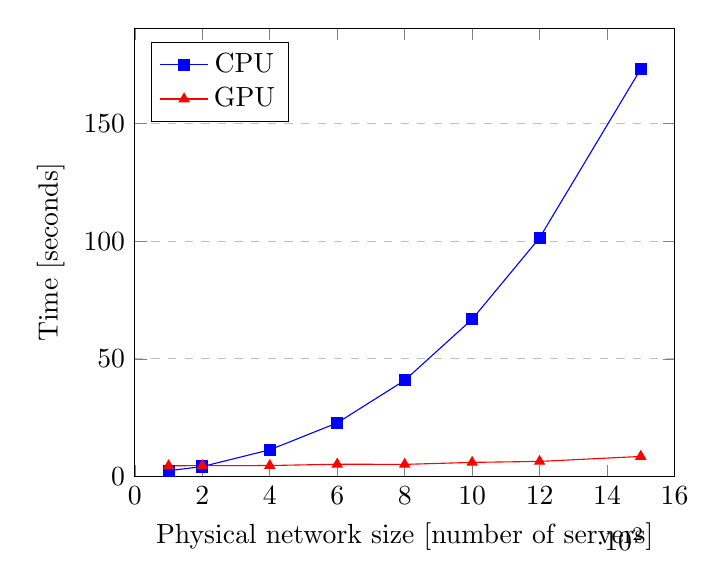
\begin{tikzpicture}
\begin{axis}[
    xlabel={Physical network size [number of servers]},
    ylabel={Time [seconds]},
    xmin=0, xmax=1600,
    ymin=0,
    % ymax=500,
    xtick={0,200,400,600,800,1000, 1200, 1400, 1600},
    % ytick={0,100,200,300,400,500},
    legend pos=north west,
    ymajorgrids=true,
    grid style=dashed,
    scaled x ticks=base 10:-2,
    % width=\linewidth,
    % height=0.5\linewidth,
]

\addplot[
    color=blue,
    mark=square*,
    ]
    coordinates {
(100,2.4853391647338867)
(200,4.235361337661743)
(400,11.350443363189697)
(600,22.781522274017334)
(800,40.86129117012024)
(1000,66.8314619064331)
(1200,101.40787291526794)
(1500,173.1523768901825)
    };
\addlegendentry{CPU}

\addplot[
    color=red,
    mark=triangle*,
    ]
    coordinates {
(100,4.573425054550171)
(200,4.64028000831604)
(400,4.674714803695679)
(600,5.2382402420043945)
(800,5.166032552719116)
(1000,6.011478662490845)
(1200,6.42925238609314)
(1500,8.54262924194336)
    };
\addlegendentry{GPU}

\end{axis}
\end{tikzpicture}
  			}%
  			\caption{
  			مقایسه زمان اجرای \lr{GPU} و \lr{CPU}
  		}
  			\label{fig:gpu-cpu-comparision}
  		\end{minipage}\hfill
  		\begin{minipage}[t]{.48\linewidth}
  			\centering
  			\resizebox{\linewidth}{!}{%
  				% This file was created by tikzplotlib v0.9.2.
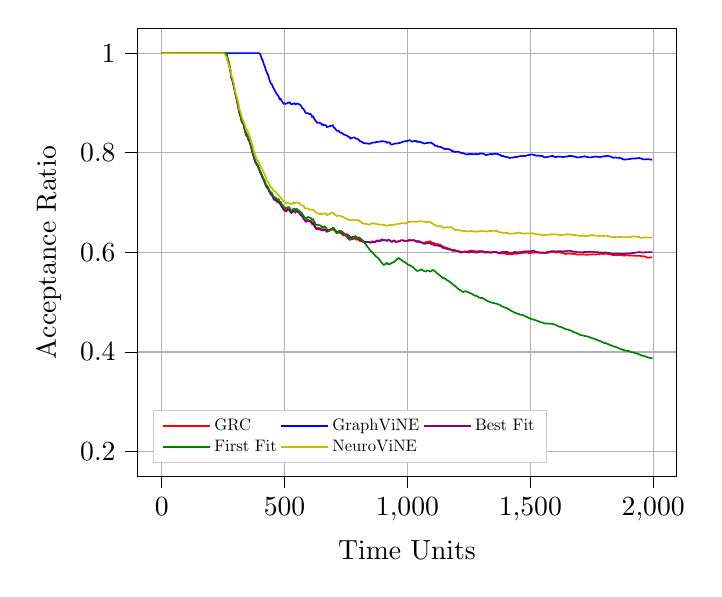
\begin{tikzpicture}

\definecolor{color0}{rgb}{0.501960784313725,0,0.501960784313725}
\definecolor{color1}{rgb}{0.75,0.75,0}

\begin{axis}[
legend cell align={left},
legend style={ fill opacity=1, draw opacity=1, text opacity=1, draw=white!80!black, legend columns=3,nodes={scale=0.6, transform shape}},
tick align=outside,
tick pos=left,
x grid style={white!69.0196078431373!black},
xlabel={Time Units},
xmin=-99.8, xmax=2095.8,
xtick style={color=black},
y grid style={white!69.0196078431373!black},
ylabel={Acceptance Ratio},
ymin=0.15,  ymax=1.05,
ytick style={color=black},
ytick={0.2,0.4,0.6,0.8,1},
yticklabels={0.2,0.4,0.6,0.8,1},
ymajorgrids=true,
xmajorgrids=true,
legend pos=south west,
% width=\linewidth,
% height=0.5\linewidth,
]
\addplot [semithick, red]
table {%
0 1
4 1
8 1
12 1
16 1
20 1
24 1
28 1
32 1
36 1
40 1
44 1
48 1
52 1
56 1
60 1
64 1
68 1
72 1
76 1
80 1
84 1
88 1
92 1
96 1
100 1
104 1
108 1
112 1
116 1
120 1
124 1
128 1
132 1
136 1
140 1
144 1
148 1
152 1
156 1
160 1
164 1
168 1
172 1
176 1
180 1
184 1
188 1
192 1
196 1
200 1
204 1
208 1
212 1
216 1
220 1
224 1
228 1
232 1
236 1
240 1
244 1
248 1
252 1
256 1
260 1
264 0.998116760828625
268 0.98886827458256
272 0.981718464351006
276 0.972972972972973
280 0.962699822380107
284 0.949211908931699
288 0.946459412780656
292 0.936967632027257
296 0.927731092436975
300 0.917081260364842
304 0.909983633387889
308 0.901453957996769
312 0.891547049441786
316 0.880314960629921
320 0.87402799377916
324 0.8678955453149
328 0.860394537177542
332 0.859070464767616
336 0.85037037037037
340 0.841874084919473
344 0.835021707670043
348 0.834048640915594
352 0.827439886845827
356 0.823776223776224
360 0.81881051175657
364 0.811217510259918
368 0.803788903924222
372 0.796519410977242
376 0.789403973509934
380 0.782437745740498
384 0.778210116731518
388 0.775353016688062
392 0.772554002541296
396 0.767295597484277
400 0.76214196762142
404 0.759556103575832
408 0.753357753357753
412 0.749697702539299
416 0.744910179640718
420 0.740213523131673
424 0.734430082256169
428 0.732246798603027
432 0.730103806228374
436 0.725714285714286
440 0.721404303510759
444 0.718294051627385
448 0.717463848720801
452 0.713340683572216
456 0.708196721311475
460 0.707475622968581
464 0.706766917293233
468 0.703940362087327
472 0.703273495248152
476 0.70261780104712
480 0.699896157840083
484 0.698249227600412
488 0.693564862104188
492 0.691995947315096
496 0.688442211055276
500 0.686939182452642
504 0.685459940652819
508 0.685966633954858
512 0.687439143135346
516 0.68695652173913
520 0.686481303930968
524 0.68220742150333
528 0.680830972615675
532 0.682286785379569
536 0.684651162790698
540 0.685133887349954
544 0.68102658111824
548 0.683348498635123
552 0.682926829268293
556 0.680717488789238
560 0.680320569902048
564 0.677276746242264
568 0.675153643546971
572 0.673060156931125
576 0.67012987012987
580 0.667239896818573
584 0.664389410760034
588 0.662425784563189
592 0.664700926705981
596 0.665271966527197
600 0.664172901080632
604 0.663088356729975
608 0.662838392124692
612 0.658516707416463
616 0.659919028340081
620 0.655671761866452
624 0.653077537969624
628 0.649722001588562
632 0.648776637726914
636 0.649411764705882
640 0.648480124707716
644 0.648334624322231
648 0.647421093148576
652 0.644988523335884
656 0.64638783269962
660 0.64474678760393
664 0.646130728775357
668 0.645257654966393
672 0.642910170749814
676 0.644280442804428
680 0.643433602347762
684 0.644784828592268
688 0.645395213923133
692 0.645277577505407
696 0.645878136200717
700 0.645046329294369
704 0.643515237420269
708 0.641296687808316
712 0.640504555010512
716 0.639721254355401
720 0.64033264033264
724 0.639558924879394
728 0.638793694311172
732 0.638036809815951
736 0.635254237288136
740 0.633850303438975
744 0.634473507712944
748 0.633088725817212
752 0.633045786330458
756 0.632343234323432
760 0.631648063033487
764 0.629653821032005
768 0.627030539311241
772 0.627020038784745
776 0.627009646302251
780 0.626999360204735
784 0.628262253341821
788 0.626979100696643
792 0.625708884688091
796 0.626959247648903
800 0.625077978789769
804 0.624456859093731
808 0.621988882025942
812 0.622618315918869
816 0.62262996941896
820 0.620815581253804
824 0.62023016353725
828 0.620253164556962
832 0.620275944811038
836 0.62089552238806
840 0.620915032679739
844 0.620342992312241
848 0.619776339022955
852 0.620386643233743
856 0.621574344023324
860 0.622170632617528
864 0.620450606585789
868 0.621621621621622
872 0.622781911848884
876 0.623931623931624
880 0.623936471922859
884 0.622811970638058
888 0.623946037099494
892 0.625069949636262
896 0.626183844011142
900 0.624514697726012
904 0.625069022639426
908 0.624518966465091
912 0.624521072796935
916 0.623433242506812
920 0.623982637004883
924 0.62506753106429
928 0.623991393222162
932 0.622388859132298
936 0.621333333333333
940 0.621879978757302
944 0.623479640401904
948 0.622959452343339
952 0.620870477189303
956 0.62088772845953
960 0.621944877795112
964 0.621957534955981
968 0.623001547189273
972 0.624036979969183
976 0.624040920716113
980 0.624044829342843
984 0.623541349568747
988 0.623547246083881
992 0.622546552591847
996 0.623057644110276
1000 0.623065401897154
1004 0.624564893088016
1008 0.62555720653789
1012 0.624568327577701
1016 0.623587223587224
1020 0.624082232011747
1024 0.62457337883959
1028 0.62360369111219
1032 0.622641509433962
1036 0.621204819277108
1040 0.621219395103217
1044 0.621712099473936
1048 0.620295378751787
1052 0.6203132415757
1056 0.619858156028369
1060 0.61987753179463
1064 0.618958235570155
1068 0.618980832164563
1072 0.619934792734048
1076 0.620881670533643
1080 0.62043458159963
1084 0.621372639336711
1088 0.621844882973841
1092 0.622313671696388
1096 0.620956719817768
1100 0.619609623241035
1104 0.61917684305744
1108 0.618296529968454
1112 0.616973506960036
1116 0.61744966442953
1120 0.617030762371823
1124 0.616170590848512
1128 0.615759185480301
1132 0.615791795324217
1136 0.614065934065934
1140 0.613228208497591
1144 0.611959842863378
1148 0.611135276207047
1152 0.609882964889467
1156 0.609503239740821
1160 0.609126130004305
1164 0.608322608322608
1168 0.607524583155195
1172 0.606731998295697
1176 0.60552016985138
1180 0.60431654676259
1184 0.604808097849009
1188 0.604875998318621
1192 0.604943443653121
1196 0.603757828810021
1200 0.60341240116521
1204 0.603069265864786
1208 0.602728400165358
1212 0.601977750309024
1216 0.601232032854209
1220 0.60130986492018
1224 0.600571195430437
1228 0.601057340382269
1232 0.601945683015809
1236 0.601616161616162
1240 0.601691502215062
1244 0.601766358892011
1248 0.602240896358543
1252 0.603111288392501
1256 0.602783300198807
1260 0.603646452635751
1264 0.603318846305808
1268 0.60338716029933
1272 0.602669807616804
1276 0.601956947162427
1280 0.602028872415139
1284 0.602100350058343
1288 0.602171384257464
1292 0.602628527251643
1296 0.602697495183044
1300 0.60238186707645
1304 0.602451168134814
1308 0.601374570446735
1312 0.599543205177008
1316 0.599620493358634
1320 0.599318955732123
1324 0.599773670313089
1328 0.600225648740128
1332 0.600299962504687
1336 0.599252336448598
1340 0.600074543421543
1344 0.599405425492382
1348 0.599851796961838
1352 0.60029553010713
1356 0.60036832412523
1360 0.600073448402497
1364 0.600146466495789
1368 0.599123767798467
1372 0.598471059337459
1376 0.598185117967332
1380 0.597538906985161
1384 0.597979068928185
1388 0.598056854983807
1392 0.598134194474345
1396 0.597495527728086
1400 0.597574027827328
1404 0.596229099964426
1408 0.59666548421426
1412 0.596038203042094
1416 0.596119929453263
1420 0.59655293703834
1424 0.595931252192213
1428 0.596362364463099
1432 0.597488664108825
1436 0.597913043478261
1440 0.596947624002775
1444 0.597025250778277
1448 0.597102449120386
1452 0.598211214310286
1456 0.598284734133791
1460 0.598699965788573
1464 0.598771750255885
1468 0.598843143926506
1472 0.599592806243638
1476 0.599323181049069
1480 0.599392507593655
1484 0.599798047795355
1488 0.599530043638805
1492 0.598928690994309
1496 0.597996661101836
1500 0.598734598734599
1504 0.599136499501827
1508 0.599205034779728
1512 0.599273207796498
1516 0.599670510708402
1520 0.599408478475189
1524 0.599803343166175
1528 0.599215429879045
1532 0.599608738180633
1536 0.599349593495935
1540 0.598767434317223
1544 0.599158848269169
1548 0.598902871894159
1552 0.599291921467654
1556 0.598715890850722
1560 0.598783221261607
1564 0.598530820824018
1568 0.598916852500796
1572 0.599300921512552
1576 0.599683042789223
1580 0.600063231109706
1584 0.601072216966257
1588 0.601132431582259
1592 0.600878569187324
1596 0.600312989045383
1600 0.60006244146113
1604 0.599813142323264
1608 0.599565082323703
1612 0.600247908273939
1616 0.6
1620 0.599753314831946
1624 0.599815441402645
1628 0.598956735194845
1632 0.598408325681053
1636 0.598167938931298
1640 0.597624124276576
1644 0.596779094500152
1648 0.59715065171264
1652 0.597520411248866
1656 0.597586726998492
1660 0.597351790550707
1664 0.597418192734914
1668 0.59748427672956
1672 0.596653719749029
1676 0.597317436661699
1680 0.59678858162355
1684 0.596558884603975
1688 0.595738384137319
1692 0.59551225273103
1696 0.595581737849779
1700 0.595650896267999
1704 0.595719730284374
1708 0.595788242176075
1712 0.595856434199008
1716 0.596506550218341
1720 0.59541097879756
1724 0.5954795711388
1728 0.59525874530211
1732 0.5950389385636
1736 0.595395683453237
1740 0.595750789549239
1744 0.595817817244343
1748 0.595884538439554
1752 0.596236099230111
1756 0.59601706970128
1760 0.59551518592109
1764 0.595581988105353
1768 0.595648488273524
1772 0.596278545249507
1776 0.59606188466948
1780 0.596126859388156
1784 0.596751610193223
1788 0.597652975691534
1792 0.597156398104265
1796 0.596940194714882
1800 0.596724951429364
1804 0.597341456660205
1808 0.597402597402597
1812 0.597187758478081
1816 0.596698762035763
1820 0.596211913258304
1824 0.596001095590249
1828 0.596064498496857
1832 0.595036814835015
1836 0.594285714285714
1840 0.594623947868585
1844 0.594689785965863
1848 0.594214652608813
1852 0.594550849743728
1856 0.594616419919246
1860 0.594413107708837
1864 0.594478692039668
1868 0.594811446910939
1872 0.59434214037897
1876 0.59387483355526
1880 0.593409513685889
1884 0.593476531424025
1888 0.593807885684043
1892 0.594137839978875
1896 0.593939393939394
1900 0.594267683407836
1904 0.593282602991341
1908 0.593872741555381
1912 0.593676509014894
1916 0.59348109517601
1920 0.593286494925839
1924 0.593092703193976
1928 0.59289971495206
1932 0.592966123610034
1936 0.593032258064516
1940 0.593355652845738
1944 0.593420714469288
1948 0.592716081046422
1952 0.592270284105452
1956 0.591826309067688
1960 0.592403772622993
1964 0.591961332994149
1968 0.591520690530592
1972 0.590321763364581
1976 0.589633375474083
1980 0.589200100933636
1984 0.589775875094435
1988 0.589595375722543
1992 0.589917231000752
1996 0.590488110137672
};
\addlegendentry{GRC}
\addplot [semithick, blue]
table {%
0 1
4 1
8 1
12 1
16 1
20 1
24 1
28 1
32 1
36 1
40 1
44 1
48 1
52 1
56 1
60 1
64 1
68 1
72 1
76 1
80 1
84 1
88 1
92 1
96 1
100 1
104 1
108 1
112 1
116 1
120 1
124 1
128 1
132 1
136 1
140 1
144 1
148 1
152 1
156 1
160 1
164 1
168 1
172 1
176 1
180 1
184 1
188 1
192 1
196 1
200 1
204 1
208 1
212 1
216 1
220 1
224 1
228 1
232 1
236 1
240 1
244 1
248 1
252 1
256 1
260 1
264 1
268 1
272 1
276 1
280 1
284 1
288 1
292 1
296 1
300 1
304 1
308 1
312 1
316 1
320 1
324 1
328 1
332 1
336 1
340 1
344 1
348 1
352 1
356 1
360 1
364 1
368 1
372 1
376 1
380 1
384 1
388 1
392 1
396 1
400 0.998754669987547
404 0.99383477188656
408 0.987789987789988
412 0.984280532043531
416 0.977245508982036
420 0.972716488730724
424 0.965922444183314
428 0.960419091967404
432 0.957324106113033
436 0.950857142857143
440 0.944507361268403
444 0.939393939393939
448 0.937708565072303
452 0.932745314222712
456 0.92896174863388
460 0.925243770314193
464 0.921589688506982
468 0.917997870074547
472 0.915522703273495
476 0.913089005235602
480 0.907580477673936
484 0.908341915550978
488 0.903983656792646
492 0.901722391084093
496 0.898492462311558
500 0.899302093718844
504 0.898120672601385
508 0.89892051030422
512 0.899707887049659
516 0.90048309178744
520 0.901246404602109
524 0.899143672692674
528 0.897072710103872
532 0.89784442361762
536 0.898604651162791
540 0.899353647276085
544 0.897341888175985
548 0.898089171974522
552 0.898825654923216
556 0.897757847533632
560 0.897595725734639
564 0.895667550839965
568 0.893766461808604
572 0.889276373147341
576 0.888311688311688
580 0.885640584694755
584 0.881298035866781
588 0.879558948261238
592 0.879528222409436
596 0.879497907949791
600 0.877805486284289
604 0.877786952931462
608 0.876948318293683
612 0.872045639771801
616 0.872874493927126
620 0.86886564762671
624 0.865707434052758
628 0.863383637807784
632 0.860299921073402
636 0.860392156862745
640 0.860483242400624
644 0.859798605731991
648 0.859122401847575
652 0.856159143075746
656 0.857034220532319
660 0.854875283446712
664 0.855747558226897
668 0.855115758028379
672 0.851521900519673
676 0.85239852398524
680 0.852531181217902
684 0.853391684901532
688 0.854242204496012
692 0.85436193222783
696 0.855197132616487
700 0.851033499643621
704 0.84975194897236
708 0.84707540521494
712 0.844428871758935
716 0.84390243902439
720 0.844074844074844
724 0.841488628532047
728 0.840301576422207
732 0.839809134287662
736 0.83864406779661
740 0.836817262306136
744 0.836351441985245
748 0.835223482321548
752 0.834771068347711
756 0.833663366336634
760 0.831910702560735
764 0.8314826910516
768 0.828460038986355
772 0.82934712346477
776 0.830225080385852
780 0.830454254638516
784 0.830681094844048
788 0.829005699810006
792 0.827977315689981
796 0.828213166144201
800 0.826575171553337
804 0.824953445065177
808 0.822730080296479
812 0.822372464658881
816 0.822018348623853
820 0.819841752891053
824 0.818897637795276
828 0.819168173598553
832 0.818836232753449
836 0.818507462686567
840 0.818775995246584
844 0.81785925487877
848 0.818128310771042
852 0.818980667838313
856 0.819825072886297
860 0.820661636680209
864 0.820335066435586
868 0.820586543990799
872 0.821408128219805
876 0.821652421652422
880 0.821894498014748
884 0.822134387351779
888 0.822372119168072
892 0.822607722439843
896 0.823398328690808
900 0.823072656683306
904 0.822749861954721
908 0.822429906542056
912 0.822112753147236
916 0.82016348773842
920 0.820401519262073
924 0.82117774176121
928 0.820333512641205
932 0.8168184252812
936 0.816533333333333
940 0.816781731279873
944 0.817556848228451
948 0.818325434439178
952 0.818563188253802
956 0.818276762402089
960 0.819032761310452
964 0.819264629725531
968 0.819494584837545
972 0.820236260914227
976 0.820971867007673
980 0.821701477330616
984 0.822425164890918
988 0.823143001515917
992 0.823351786612984
996 0.823057644110276
1000 0.823764353469795
1004 0.824465440079562
1008 0.825160970777613
1012 0.82486433152442
1016 0.822604422604423
1020 0.822320117474302
1024 0.823013164310093
1028 0.823700825643516
1032 0.823415578132559
1036 0.823614457831325
1040 0.821891502640422
1044 0.822572931611669
1048 0.821343496903287
1052 0.821547223540579
1056 0.821276595744681
1060 0.820065944418276
1064 0.819333646175505
1068 0.818606825619448
1072 0.818816953889148
1076 0.819489559164733
1080 0.819232547387887
1084 0.819898664210041
1088 0.820100963744837
1092 0.820301783264746
1096 0.820501138952164
1100 0.818883340898774
1104 0.817729534147445
1108 0.816584046867959
1112 0.814099685675797
1116 0.813870246085011
1120 0.814088274632189
1124 0.812083518436251
1128 0.81186365648517
1132 0.812086457873842
1136 0.811428571428571
1140 0.810775295663601
1144 0.809253601047577
1148 0.808612440191388
1152 0.807108799306459
1156 0.807775377969762
1160 0.808006887645286
1164 0.807807807807808
1168 0.806755023514322
1172 0.806561567959097
1176 0.80552016985138
1180 0.803639441388066
1184 0.803880219316744
1188 0.802017654476671
1192 0.80184331797235
1196 0.80125260960334
1200 0.801914273824386
1204 0.801742015761095
1208 0.801984291029351
1212 0.800988875154512
1216 0.8
1220 0.799426934097421
1224 0.800081599347205
1228 0.798698657991053
1232 0.79813538710985
1236 0.797171717171717
1240 0.796616995569875
1244 0.796868727418707
1248 0.797118847539016
1252 0.797766254487435
1256 0.796819085487078
1260 0.797463337296869
1264 0.797313314895298
1268 0.797164237888933
1272 0.797016097369454
1276 0.797260273972603
1280 0.797502926258291
1284 0.796966161026838
1288 0.797208220240403
1292 0.797835330498647
1296 0.798458574181118
1300 0.798693814829043
1304 0.798544618919954
1308 0.798014509354716
1312 0.797106966121051
1316 0.796204933586338
1320 0.795308361710178
1324 0.795926065635609
1328 0.796540052651373
1332 0.796775403074616
1336 0.797009345794393
1340 0.797614610510622
1344 0.796729840208101
1348 0.797332345313079
1352 0.797931289250092
1356 0.798158379373849
1360 0.797649651120088
1364 0.797876235811058
1368 0.7973713033954
1372 0.79614124499454
1376 0.795644283121597
1380 0.794788273615635
1384 0.793215445687477
1388 0.793810723281756
1392 0.792967348403301
1396 0.791771019677996
1400 0.792008562254727
1404 0.791177516897901
1408 0.791060659808443
1412 0.790237000353732
1416 0.789417989417989
1420 0.790010552233556
1424 0.790249035426166
1428 0.790136411332634
1432 0.790722009068713
1436 0.791304347826087
1440 0.791536593825876
1444 0.791421653407126
1448 0.791997240427734
1452 0.792569659442725
1456 0.792795883361921
1460 0.793362983236401
1464 0.792903445922893
1468 0.79346716570262
1472 0.794027824906685
1476 0.793231810490694
1480 0.79379007762403
1484 0.794345338269943
1488 0.794897616649882
1492 0.795446936725812
1496 0.795659432387312
1500 0.796203796203796
1504 0.796745267353039
1508 0.796621397813846
1512 0.79616782292699
1516 0.795387149917628
1520 0.794610581662833
1524 0.794165847263192
1528 0.794050343249428
1532 0.794587544832083
1536 0.793821138211382
1540 0.79403178722024
1544 0.793594306049822
1548 0.793481768312359
1552 0.792726102349533
1556 0.791011235955056
1560 0.791226384886327
1564 0.79112104758863
1568 0.791334820006371
1572 0.791865268509692
1576 0.792076069730586
1580 0.792601960164401
1584 0.793125197098707
1588 0.793645800566216
1592 0.793536240978977
1596 0.792175273865415
1600 0.791757727130815
1604 0.791342260977889
1608 0.791860826343585
1612 0.792376820576387
1616 0.79258114374034
1620 0.791859389454209
1624 0.792371577976007
1628 0.79165388155876
1632 0.791245791245791
1636 0.791450381679389
1640 0.791958574474566
1644 0.791856578547554
1648 0.79236132161261
1652 0.792863622618688
1656 0.793363499245852
1660 0.793560036111947
1664 0.793455418793155
1668 0.793351302785265
1672 0.79265013444876
1676 0.792846497764531
1680 0.791852512637526
1684 0.792049836843667
1688 0.79106244451021
1692 0.790670209625037
1696 0.790574374079529
1700 0.790772847487511
1704 0.791263559073585
1708 0.79175197426148
1712 0.791946308724832
1716 0.792430858806405
1720 0.79291315713041
1724 0.79252390611417
1728 0.7918473547268
1732 0.791173925584078
1736 0.791079136690647
1740 0.790697674418605
1744 0.790604411343455
1748 0.790797370677336
1752 0.791274593669803
1756 0.791749644381223
1760 0.792222537609992
1764 0.792410082129708
1768 0.791749081661486
1772 0.791936848040598
1776 0.792123769338959
1780 0.791187201796239
1784 0.7913749649958
1788 0.791841296451523
1792 0.792305547811542
1796 0.792489568845619
1800 0.792672772689425
1804 0.793132096372196
1808 0.79358938933407
1812 0.793768955059278
1816 0.793397524071527
1820 0.793027724402965
1824 0.792659545330047
1828 0.792566274938508
1832 0.791109899100082
1836 0.789931972789116
1840 0.790116752647298
1844 0.790300731509076
1848 0.790483914571506
1852 0.789857027245751
1856 0.789771197846568
1860 0.789685737308622
1864 0.78960064325918
1868 0.789248462155657
1872 0.788097144382172
1876 0.787217043941411
1880 0.786606431039065
1884 0.786263590559533
1888 0.786451442180471
1892 0.786638500132031
1896 0.786824769433465
1900 0.787010255061793
1904 0.787457360272894
1908 0.78790259230165
1912 0.788084661614842
1916 0.788526727509778
1920 0.788186312776477
1924 0.788366658010906
1928 0.788546255506608
1932 0.788983708301009
1936 0.788903225806452
1940 0.789080607777492
1944 0.789514263685428
1948 0.788407283918954
1952 0.788328640900947
1956 0.787484035759898
1960 0.786897782309457
1964 0.78656830323073
1968 0.786747905559787
1972 0.787180136812769
1976 0.78685208596713
1980 0.786777693666414
1984 0.786955426844623
1988 0.786378487057049
1992 0.786054677702533
1996 0.78648310387985
};
\addlegendentry{GraphViNE}
\addplot [semithick, color0]
table {%
0 1
4 1
8 1
12 1
16 1
20 1
24 1
28 1
32 1
36 1
40 1
44 1
48 1
52 1
56 1
60 1
64 1
68 1
72 1
76 1
80 1
84 1
88 1
92 1
96 1
100 1
104 1
108 1
112 1
116 1
120 1
124 1
128 1
132 1
136 1
140 1
144 1
148 1
152 1
156 1
160 1
164 1
168 1
172 1
176 1
180 1
184 1
188 1
192 1
196 1
200 1
204 1
208 1
212 1
216 1
220 1
224 1
228 1
232 1
236 1
240 1
244 1
248 1
252 1
256 1
260 1
264 0.998116760828625
268 0.98886827458256
272 0.981718464351006
276 0.974774774774775
280 0.962699822380107
284 0.949211908931699
288 0.944732297063903
292 0.936967632027257
296 0.927731092436975
300 0.917081260364842
304 0.909983633387889
308 0.89983844911147
312 0.889952153110048
316 0.880314960629921
320 0.87402799377916
324 0.864823348694316
328 0.860394537177542
332 0.859070464767616
336 0.85037037037037
340 0.841874084919473
344 0.835021707670043
348 0.832618025751073
352 0.827439886845827
356 0.823776223776224
360 0.81881051175657
364 0.811217510259918
368 0.803788903924222
372 0.796519410977242
376 0.789403973509934
380 0.782437745740498
384 0.778210116731518
388 0.775353016688062
392 0.772554002541296
396 0.767295597484277
400 0.760896637608966
404 0.758323057953144
408 0.752136752136752
412 0.748488512696493
416 0.743712574850299
420 0.739027283511269
424 0.733254994124559
428 0.729918509895227
432 0.728950403690888
436 0.723428571428571
440 0.720271800679502
444 0.716049382716049
448 0.71523915461624
452 0.711135611907387
456 0.706010928961749
460 0.705308775731311
464 0.704618689581096
468 0.701810436634718
472 0.701161562829989
476 0.700523560209424
480 0.697819314641745
484 0.696189495365602
488 0.691521961184883
492 0.689969604863222
496 0.685427135678392
500 0.6839481555334
504 0.682492581602374
508 0.683022571148185
512 0.684518013631938
516 0.685024154589372
520 0.685522531160115
524 0.680304471931494
528 0.678942398489141
532 0.680412371134021
536 0.682790697674419
540 0.682363804247461
544 0.680109990834097
548 0.682438580527753
552 0.682023486901536
556 0.679820627802691
560 0.679430097951915
564 0.675508399646331
568 0.673397717295874
572 0.672188317349608
576 0.668398268398268
580 0.665520206362855
584 0.66268146883006
588 0.661577608142494
592 0.66301600673968
596 0.663598326359833
600 0.662510390689942
604 0.661436829066887
608 0.660377358490566
612 0.656886715566422
616 0.6582995951417
620 0.654062751407884
624 0.650679456434852
628 0.647339158061954
632 0.646408839779006
636 0.647058823529412
640 0.64614185502728
644 0.646785437645236
648 0.645111624326405
652 0.644223412394797
656 0.645627376425856
660 0.643990929705215
664 0.645379413974455
668 0.643764002987304
672 0.641425389755011
676 0.64280442804428
680 0.643433602347762
684 0.645514223194748
688 0.646845540246555
692 0.647440519105984
696 0.648745519713262
700 0.647897362794013
704 0.645641389085755
708 0.643410852713178
712 0.641205325858444
716 0.641114982578397
720 0.642411642411642
724 0.640937284631289
728 0.640849897189856
732 0.640081799591002
736 0.63864406779661
740 0.637221847606204
744 0.637156270959088
748 0.635757171447632
752 0.636363636363636
756 0.635643564356436
760 0.634274458305975
764 0.63226649248857
768 0.62962962962963
772 0.630252100840336
776 0.630868167202572
780 0.630838131797825
784 0.631444939528963
788 0.630145661811273
792 0.629489603024575
796 0.629467084639498
800 0.628197130380536
804 0.626939788950962
808 0.624459542927733
812 0.624462200368777
816 0.623853211009174
820 0.622641509433962
824 0.621441550575409
828 0.620855937311634
832 0.620875824835033
836 0.62089552238806
840 0.620915032679739
844 0.620342992312241
848 0.619776339022955
852 0.619800820152314
856 0.620991253644315
860 0.621009866511898
864 0.620450606585789
868 0.620471535365152
872 0.621637092157985
876 0.622792022792023
880 0.623369256948383
884 0.622247317899492
888 0.622821810005621
892 0.623391158365976
896 0.625069637883008
900 0.62396006655574
904 0.62451684152402
908 0.624518966465091
912 0.623973727422003
916 0.623433242506812
920 0.623982637004883
924 0.625607779578606
928 0.623991393222162
932 0.622388859132298
936 0.621333333333333
940 0.622411046202868
944 0.624008461131676
948 0.623486045286993
952 0.620870477189303
956 0.621409921671018
960 0.621944877795112
964 0.621957534955981
968 0.622485817431666
972 0.623523369286081
976 0.624552429667519
980 0.624554253693327
984 0.623033992897007
988 0.623547246083881
992 0.623049823855058
996 0.623057644110276
1000 0.623065401897154
1004 0.623073097961213
1008 0.623576027736503
1012 0.624568327577701
1016 0.624078624078624
1020 0.624082232011747
1024 0.625060945880058
1028 0.62408936376882
1032 0.623609095307209
1036 0.622650602409639
1040 0.621699471915506
1044 0.623146819703491
1048 0.62172463077656
1052 0.621737066919791
1056 0.620330969267139
1060 0.619406500235516
1064 0.618019709056781
1068 0.61711079943899
1072 0.617140195621798
1076 0.618097447795824
1080 0.618122977346278
1084 0.61906955320129
1088 0.61863240018357
1092 0.618655692729767
1096 0.616856492027335
1100 0.615978211529732
1104 0.615558570782451
1108 0.615141955835962
1112 0.6138302649304
1116 0.613870246085011
1120 0.61435577351761
1124 0.613505108840515
1128 0.612660469234174
1132 0.613586237318041
1136 0.611868131868132
1140 0.61060008760403
1144 0.608904408555216
1148 0.609395389299696
1152 0.607715648027742
1156 0.607775377969762
1160 0.607404218682738
1164 0.606606606606607
1168 0.605814450619923
1172 0.605879846612697
1176 0.60552016985138
1180 0.60431654676259
1184 0.603121045972164
1188 0.603194619588062
1192 0.603267700041894
1196 0.602922755741127
1200 0.602996254681648
1204 0.602654500207383
1208 0.601901612236461
1212 0.600741656365884
1216 0.59958932238193
1220 0.599672533769955
1224 0.60016319869441
1228 0.600650671004473
1232 0.601540332387515
1236 0.600808080808081
1240 0.600483286347161
1244 0.600160578081092
1248 0.59983993597439
1252 0.599920223374551
1256 0.600397614314115
1260 0.601268331351566
1264 0.600553141050968
1268 0.600236313509256
1272 0.600314095013742
1276 0.599608610567515
1280 0.599687865782286
1284 0.599766627771295
1288 0.599844901124467
1292 0.601082334750676
1296 0.601156069364162
1300 0.601229350749136
1304 0.602068173113749
1308 0.601756395570828
1312 0.601065854586981
1316 0.600759013282733
1320 0.601210745365115
1324 0.600528102602791
1328 0.600601729973674
1332 0.600299962504687
1336 0.599626168224299
1340 0.600074543421543
1344 0.600520252694166
1348 0.600592812152649
1352 0.601034355374954
1356 0.60073664825046
1360 0.600440690414983
1364 0.600146466495789
1368 0.599123767798467
1372 0.599199126319621
1376 0.599637023593466
1380 0.600072385088672
1384 0.600144352219415
1388 0.600575746671465
1392 0.601004664513814
1396 0.600715563506261
1400 0.600784873349982
1404 0.6008537886873
1408 0.60056757715502
1412 0.59957552175451
1416 0.598941798941799
1420 0.599366865986634
1424 0.599088039284462
1428 0.599160545645331
1432 0.600279037321242
1436 0.60104347826087
1440 0.600416233090531
1444 0.600138360428917
1448 0.599862021386685
1452 0.60061919504644
1456 0.600343053173242
1460 0.600410537119398
1464 0.601160013647219
1468 0.601224906430759
1472 0.601968103155752
1476 0.601692047377327
1480 0.602092473844077
1484 0.602154156849546
1488 0.60187982544478
1492 0.602276531637094
1496 0.602003338898164
1500 0.602397602397602
1504 0.602789770840252
1508 0.60284862537264
1512 0.603237528906508
1516 0.602965403624382
1520 0.601708839960565
1524 0.601442150114716
1528 0.600523046747303
1532 0.600260841212912
1536 0.6
1540 0.600064871878041
1544 0.599805888062116
1548 0.599870926105195
1552 0.599613775345993
1556 0.599036918138042
1560 0.599423631123919
1564 0.599808367933568
1568 0.600509716470213
1572 0.600889736256752
1576 0.60095087163233
1580 0.601644008852355
1584 0.602018290760013
1588 0.602390688895879
1592 0.602133668026357
1596 0.602190923317684
1600 0.602247892600687
1604 0.601993148551853
1608 0.602050326188257
1612 0.602107220328479
1616 0.602472952086553
1620 0.602220166512488
1624 0.602276222700707
1628 0.60202516109236
1632 0.601469237832874
1636 0.602137404580153
1640 0.602193116052391
1644 0.602552415679125
1648 0.602606850560776
1652 0.602963410946477
1656 0.603016591251885
1660 0.603069515498044
1664 0.602521765235665
1668 0.602575621443546
1672 0.601732895129967
1676 0.601788375558867
1680 0.601248884924175
1684 0.601305250667458
1688 0.600769458419651
1692 0.600236197224683
1696 0.600294550810015
1700 0.600352630032324
1704 0.600410436822046
1708 0.599883006727113
1712 0.600525240735337
1716 0.600582241630277
1720 0.600638977635783
1724 0.600985221674877
1728 0.600751662330153
1732 0.600519180847995
1736 0.600863309352518
1740 0.60120585701981
1744 0.600973932970496
1748 0.601314661331809
1752 0.601083547191332
1756 0.601137980085348
1760 0.600624467783139
1764 0.600396488246955
1768 0.600169539417915
1772 0.600789399492529
1776 0.6
1780 0.599494807746281
1784 0.599831979837581
1788 0.599608829281922
1792 0.599665458600502
1796 0.599165507649513
1800 0.599500416319733
1804 0.600110772639158
1808 0.599889472229898
1812 0.599117728149986
1816 0.599449793672627
1820 0.598956903650837
1824 0.597918378526431
1828 0.597430992074337
1832 0.597218434687756
1836 0.596734693877551
1840 0.597339125712734
1844 0.597128149552967
1848 0.597188429305218
1852 0.597248448880496
1856 0.597577388963661
1860 0.597367714208971
1864 0.597158938622353
1868 0.597485958812517
1872 0.597010942087003
1876 0.596537949400799
1880 0.596864204092479
1884 0.596658711217184
1888 0.597247949192908
1892 0.597834697649855
1896 0.597628458498024
1900 0.59742308703655
1904 0.597743374442404
1908 0.598062319979052
1912 0.598379932061667
1916 0.598696219035202
1920 0.598750975800156
1924 0.599065177875876
1928 0.599378077222078
1932 0.599948280320662
1936 0.6
1940 0.60056657223796
1944 0.600616808018504
1948 0.600153885611695
1952 0.599948809828513
1956 0.599744572158365
1960 0.600050981391792
1964 0.59959297888578
1968 0.6001523229246
1972 0.600202685583988
1976 0.6
1980 0.600302800908403
1984 0.600604381767817
1988 0.600402111083187
1992 0.600451467268623
1996 0.600750938673342
};
\addlegendentry{Best Fit}
\addplot [semithick, green!50.1960784313725!black]
table {%
0 1
4 1
8 1
12 1
16 1
20 1
24 1
28 1
32 1
36 1
40 1
44 1
48 1
52 1
56 1
60 1
64 1
68 1
72 1
76 1
80 1
84 1
88 1
92 1
96 1
100 1
104 1
108 1
112 1
116 1
120 1
124 1
128 1
132 1
136 1
140 1
144 1
148 1
152 1
156 1
160 1
164 1
168 1
172 1
176 1
180 1
184 1
188 1
192 1
196 1
200 1
204 1
208 1
212 1
216 1
220 1
224 1
228 1
232 1
236 1
240 1
244 1
248 1
252 1
256 1
260 1
264 1
268 0.990723562152134
272 0.983546617915905
276 0.974774774774775
280 0.964476021314387
284 0.950963222416813
288 0.946459412780656
292 0.936967632027257
296 0.927731092436975
300 0.918739635157546
304 0.911620294599018
308 0.903069466882068
312 0.893141945773525
316 0.883464566929134
320 0.877138413685848
324 0.869431643625192
328 0.861911987860394
332 0.860569715142429
336 0.851851851851852
340 0.844802342606149
344 0.837916063675832
348 0.836909871244635
352 0.83026874115983
356 0.826573426573427
360 0.821576763485477
364 0.813953488372093
368 0.806495263870095
372 0.799196787148594
376 0.79205298013245
380 0.785058977719528
384 0.780804150453956
388 0.777920410783055
392 0.773824650571792
396 0.768553459119497
400 0.763387297633873
404 0.76078914919852
408 0.754578754578755
412 0.750906892382104
416 0.746107784431138
420 0.742586002372479
424 0.735605170387779
428 0.733410942956927
432 0.731257208765859
436 0.726857142857143
440 0.723669309173273
444 0.720538720538721
448 0.719688542825361
452 0.715545755237045
456 0.711475409836066
460 0.710725893824485
464 0.709989258861439
468 0.707135250266241
472 0.706441393875396
476 0.706806282722513
480 0.701973001038422
484 0.701338825952626
488 0.696629213483146
492 0.695035460992908
496 0.691457286432161
500 0.689930209371884
504 0.688427299703264
508 0.688910696761531
512 0.690360272638754
516 0.690821256038647
520 0.690316395014382
524 0.685061845861085
528 0.683663833805477
532 0.685098406747891
536 0.687441860465116
540 0.687903970452447
544 0.684692942254812
548 0.686988171064604
552 0.686540198735321
556 0.684304932735426
560 0.683882457702582
564 0.680813439434129
568 0.680421422300263
572 0.67741935483871
576 0.674458874458874
580 0.671539122957868
584 0.66865926558497
588 0.667514843087362
592 0.669755686604886
596 0.671129707112971
600 0.669991687448046
604 0.669694467382329
608 0.668580803937654
612 0.665036674816626
616 0.666396761133603
620 0.662107803700724
624 0.658673061550759
628 0.655281969817315
632 0.655090765588003
636 0.655686274509804
640 0.654715510522214
644 0.654531371030209
648 0.652809853733641
652 0.650344299923489
656 0.65171102661597
660 0.650037792894936
664 0.652141247182569
668 0.649738610903659
672 0.646622123236823
676 0.645756457564576
680 0.643433602347762
684 0.643326039387309
688 0.645395213923133
692 0.647440519105984
696 0.649462365591398
700 0.649322879543835
704 0.645641389085755
708 0.64200140944327
712 0.638402242466713
716 0.639024390243902
720 0.641025641025641
724 0.643004824259132
728 0.642220699108979
732 0.642808452624404
736 0.640677966101695
740 0.639244774106541
744 0.637156270959088
748 0.634422948632422
752 0.631718646317186
756 0.62970297029703
760 0.627051871306632
764 0.625081645983018
768 0.62508122157245
772 0.627020038784745
776 0.627652733118971
780 0.62891874600128
784 0.630808402291534
788 0.632678910702977
792 0.630749842470069
796 0.629467084639498
800 0.630068621334997
804 0.630043451272501
808 0.627547869054972
812 0.626920712968654
816 0.623853211009174
820 0.620815581253804
824 0.62023016353725
828 0.617239300783605
832 0.615476904619076
836 0.612537313432836
840 0.609625668449198
844 0.606741573033708
848 0.604473219540906
852 0.601640304628002
856 0.600583090379009
860 0.598374927452118
864 0.596187175043328
868 0.59401955146636
872 0.591871780194619
876 0.59031339031339
880 0.588769143505389
884 0.586674195369848
888 0.584035975267004
892 0.581421376608842
896 0.57883008356546
900 0.576261785912368
904 0.574820541137493
908 0.575590984057174
912 0.577449370552819
916 0.57874659400545
920 0.57677699403147
924 0.57590491626148
928 0.576116191500807
932 0.577932512051419
936 0.578666666666667
940 0.579925650557621
944 0.58011634056055
948 0.581885202738283
952 0.583639223911903
956 0.585378590078329
960 0.587103484139366
964 0.588814085965821
968 0.586900464156782
972 0.58602978941962
976 0.584654731457801
980 0.582781456953642
984 0.581938102486048
988 0.580596260737746
992 0.579265223955712
996 0.577944862155388
1000 0.576135796305542
1004 0.575335653903531
1008 0.574046557701833
1012 0.573754316724223
1016 0.571498771498771
1020 0.571708272148801
1024 0.569478303266699
1028 0.567265662943176
1032 0.565553942912433
1036 0.563855421686747
1040 0.562650024003841
1044 0.56336681013869
1048 0.56360171510243
1052 0.564784053156146
1056 0.565957446808511
1060 0.564766839378238
1064 0.563585171281089
1068 0.562412342215989
1072 0.56171401956218
1076 0.561948955916473
1080 0.563569116967175
1084 0.56333486872409
1088 0.56264341441028
1092 0.561499771376315
1096 0.562186788154897
1100 0.563776668179755
1104 0.564450474898236
1108 0.563316809373592
1112 0.562191288729232
1116 0.560178970917226
1120 0.558181007579135
1124 0.556641492669924
1128 0.555112881806109
1132 0.553595059550066
1136 0.552087912087912
1140 0.550153307052124
1144 0.548668703622872
1148 0.54849934754241
1152 0.547030775899436
1156 0.546436285097192
1160 0.544554455445545
1164 0.543543543543544
1168 0.54211201368106
1172 0.54069024286323
1176 0.53927813163482
1180 0.537875581887431
1184 0.536060733867566
1188 0.534258091635141
1192 0.533305404273146
1196 0.531524008350731
1200 0.529754473574698
1204 0.527996681874741
1208 0.526250516742456
1212 0.524515863205604
1216 0.524024640657084
1220 0.522308636921818
1224 0.521011831905345
1228 0.520536803578691
1232 0.521686258613701
1236 0.522020202020202
1240 0.521546516310914
1244 0.520272982737856
1248 0.519407763105242
1252 0.51934583167132
1256 0.517693836978131
1260 0.517637732857709
1264 0.516001580403003
1268 0.514769594328476
1272 0.513937966234786
1276 0.512720156555773
1280 0.512680452594616
1284 0.511863088292493
1288 0.510663047692904
1292 0.509083880943177
1296 0.508670520231214
1300 0.508259700345755
1304 0.509000382995021
1308 0.507445589919817
1312 0.50628092881614
1316 0.505123339658444
1320 0.503972758229285
1324 0.503206337231233
1328 0.501692365550959
1332 0.500937382827147
1336 0.500560747663551
1340 0.499440924338427
1344 0.498699368264586
1348 0.49870322341608
1352 0.498337643147396
1356 0.497605893186004
1360 0.497245684906353
1364 0.496887586964482
1368 0.495801387367652
1372 0.495449581361485
1376 0.49437386569873
1380 0.492942453854506
1384 0.491880187657885
1388 0.490824037423534
1392 0.490132759239325
1396 0.489445438282648
1400 0.48876204067071
1404 0.488082532906439
1408 0.487052146151117
1412 0.486027591085957
1416 0.484656084656085
1420 0.483292296869504
1424 0.482286916871273
1428 0.481287163343826
1432 0.480292989187304
1436 0.47895652173913
1440 0.478321193201526
1444 0.477689380837081
1448 0.476716109003105
1452 0.476780185758514
1456 0.475471698113208
1460 0.47485460143688
1464 0.474582053906517
1468 0.473970738346376
1472 0.473702069901595
1476 0.472419627749577
1480 0.471481606479919
1484 0.47088522383036
1488 0.469956361195032
1492 0.468697689989956
1496 0.467779632721202
1500 0.467199467199467
1504 0.465958153437396
1508 0.46538588936734
1512 0.465147010241163
1516 0.46490939044481
1520 0.463687150837989
1524 0.463454605047525
1528 0.462569467146126
1532 0.462014998369742
1536 0.461138211382114
1540 0.459941615309763
1544 0.459721772889033
1548 0.45918038076799
1552 0.458641776633408
1556 0.457784911717496
1560 0.457252641690682
1564 0.457042478441393
1568 0.457470532016566
1572 0.457260883380998
1576 0.456418383518225
1580 0.456528612077142
1584 0.456638284452854
1588 0.457061969172696
1592 0.456228427988704
1596 0.455399061032864
1600 0.454886044333437
1604 0.454064154469013
1608 0.453246349798074
1612 0.4521227145956
1616 0.451004636785162
1620 0.450508788159112
1624 0.450322977545371
1628 0.449524393985885
1632 0.448729721456994
1636 0.44763358778626
1640 0.446542796222967
1644 0.445761166818596
1648 0.445286450439527
1652 0.445418808587844
1656 0.444343891402715
1660 0.443575082756545
1664 0.443110177123987
1668 0.442348008385744
1672 0.441290708096803
1676 0.440238450074516
1680 0.43919119833482
1684 0.438742212993177
1688 0.437999408108908
1692 0.436964865662828
1696 0.436229749631811
1700 0.435204231560388
1704 0.434183523893286
1708 0.433752559227844
1712 0.433323606653049
1716 0.433187772925764
1720 0.432181237293058
1724 0.432048681541582
1728 0.431627638045678
1732 0.431208537640612
1736 0.430503597122302
1740 0.430089003732415
1744 0.429103408765397
1748 0.428408116604744
1752 0.427715996578272
1756 0.427027027027027
1760 0.426341186488788
1764 0.425941659586519
1768 0.424978807572761
1772 0.424020298844094
1776 0.423066104078762
1780 0.422396856581532
1784 0.422010641276953
1788 0.421067337245041
1792 0.420128240869808
1796 0.419193324061196
1800 0.418262558978629
1804 0.418166712821933
1808 0.417518651561205
1812 0.416597739178384
1816 0.41595598349381
1820 0.415042547351084
1824 0.414133114215284
1828 0.413500956545504
1832 0.412598854649577
1836 0.411700680272109
1840 0.410806407819712
1844 0.410457870495801
1848 0.410110840767775
1852 0.409225789047748
1856 0.408344549125168
1860 0.407467096427612
1864 0.406593406593407
1868 0.405990906659535
1872 0.405124099279423
1876 0.404260985352863
1880 0.403933032155195
1884 0.403076107133386
1888 0.402752050807092
1892 0.402429363612358
1896 0.401844532279315
1900 0.402051012358664
1904 0.401207032274993
1908 0.400366588112071
1912 0.399529657695323
1916 0.399478487614081
1920 0.398646890450169
1924 0.398597766813815
1928 0.397771443379114
1932 0.397207137315749
1936 0.396387096774194
1940 0.395827968065928
1944 0.395014135183757
1948 0.394203641959477
1952 0.393396467878167
1956 0.392592592592593
1960 0.392301809839409
1964 0.391757822437039
1968 0.390962173140391
1972 0.39016974917659
1976 0.389633375474083
1980 0.388846833207166
1984 0.388315285822211
1988 0.388037195275195
1992 0.388011035866566
1996 0.387984981226533
};
\addlegendentry{First Fit}
\addplot [semithick, color1]
table {%
0 1
4 1
8 1
12 1
16 1
20 1
24 1
28 1
32 1
36 1
40 1
44 1
48 1
52 1
56 1
60 1
64 1
68 1
72 1
76 1
80 1
84 1
88 1
92 1
96 1
100 1
104 1
108 1
112 1
116 1
120 1
124 1
128 1
132 1
136 1
140 1
144 1
148 1
152 1
156 1
160 1
164 1
168 1
172 1
176 1
180 1
184 1
188 1
192 1
196 1
200 1
204 1
208 1
212 1
216 1
220 1
224 1
228 1
232 1
236 1
240 1
244 1
248 1
252 1
256 0.998058252427184
260 0.994263862332696
264 0.992467043314501
268 0.98330241187384
272 0.978062157221207
276 0.971171171171171
280 0.966252220248668
284 0.95446584938704
288 0.949913644214162
292 0.942078364565588
296 0.932773109243697
300 0.920398009950249
304 0.914893617021277
308 0.907915993537964
312 0.899521531100478
316 0.888188976377953
320 0.883359253499222
324 0.875576036866359
328 0.867981790591806
332 0.865067466266867
336 0.859259259259259
340 0.855051244509517
344 0.846599131693198
348 0.84549356223176
352 0.84016973125884
356 0.836363636363636
360 0.831258644536653
364 0.822161422708618
368 0.817320703653586
372 0.809906291834003
376 0.801324503311258
380 0.795543905635649
384 0.791180285343709
388 0.785622593068036
392 0.783989834815756
396 0.779874213836478
400 0.774595267745953
404 0.769420468557337
408 0.768009768009768
412 0.764207980652962
416 0.759281437125748
420 0.755634638196916
424 0.749706227967098
428 0.745052386495926
432 0.741637831603229
436 0.738285714285714
440 0.734994337485844
444 0.730639730639731
448 0.729699666295884
452 0.726571113561191
456 0.723497267759563
460 0.722643553629469
464 0.721804511278195
468 0.718849840255591
472 0.715945089757128
476 0.715183246073298
480 0.712357217030114
484 0.709577754891864
488 0.706843718079673
492 0.70516717325228
496 0.70251256281407
500 0.701894317048853
504 0.699307616221563
508 0.698724239450442
512 0.699123661148978
516 0.69951690821256
520 0.698945349952061
524 0.697431018078021
528 0.696883852691218
532 0.698219306466729
536 0.70046511627907
540 0.698060941828255
544 0.6993583868011
548 0.699727024567789
552 0.700090334236676
556 0.699551569506726
560 0.699020480854853
564 0.695844385499558
568 0.695346795434592
572 0.693984306887533
576 0.693506493506494
580 0.691315563198624
584 0.688300597779675
588 0.687871077184054
592 0.688289806234204
596 0.687866108786611
600 0.685785536159601
604 0.686209744013212
608 0.685808039376538
612 0.685411572942135
616 0.68582995951417
620 0.684633950120676
624 0.681854516386891
628 0.679904686258936
632 0.677979479084451
636 0.67843137254902
640 0.677318784099766
644 0.676219984508133
648 0.677444187836798
652 0.676358071920429
656 0.678326996197719
660 0.678004535147392
664 0.677685950413223
668 0.678117998506348
672 0.674832962138085
676 0.676014760147601
680 0.67571533382245
684 0.677607585703866
688 0.678752719361856
692 0.679884643114636
696 0.679569892473118
700 0.678545972915182
704 0.67611622962438
708 0.674418604651163
712 0.672740014015417
716 0.673867595818815
720 0.674289674289674
724 0.673328738800827
728 0.673063742289239
732 0.67211997273347
736 0.671186440677966
740 0.67093728927849
744 0.66934942991281
748 0.667778519012675
752 0.667551426675514
756 0.666666666666667
760 0.665134602757715
764 0.665578053559765
768 0.664717348927875
772 0.664511958629606
776 0.664308681672026
780 0.664747280870122
784 0.665181413112667
788 0.664344521849272
792 0.664146187775677
796 0.665203761755486
800 0.663755458515284
804 0.664183736809435
808 0.661519456454602
812 0.660725261216964
816 0.658715596330275
820 0.657942787583688
824 0.65778316172017
828 0.657022302591923
832 0.65746850629874
836 0.656716417910448
840 0.655971479500891
844 0.655824955647546
848 0.656268393172454
852 0.657293497363796
856 0.658892128279883
860 0.658734764944864
864 0.657423454650491
868 0.657849338700403
872 0.657126502575844
876 0.656980056980057
880 0.656267725467952
884 0.655561829474873
888 0.655986509274874
892 0.655847789591494
896 0.655710306406685
900 0.655019412090959
904 0.655438983986748
908 0.65475536008796
912 0.653530377668309
916 0.653950953678474
920 0.653825284861639
924 0.654240950837385
928 0.655728886498117
932 0.655061596143546
936 0.6544
940 0.655337227827934
944 0.655737704918033
948 0.655608214849921
952 0.656004195070792
956 0.656396866840731
960 0.65730629225169
964 0.657690315898498
968 0.657555440948943
972 0.657935285053929
976 0.658312020460358
980 0.658685685175751
984 0.658548959918823
988 0.658413340070743
992 0.657775541016608
996 0.658646616541353
1000 0.659510733899151
1004 0.660865241173546
1008 0.6617137196632
1012 0.661568820917612
1016 0.661425061425061
1020 0.661771904062653
1024 0.662116040955631
1028 0.661486158329286
1032 0.661828737300435
1036 0.661204819277109
1040 0.661545847335574
1044 0.662362505978001
1048 0.662696522153406
1052 0.662078785002373
1056 0.66241134751773
1060 0.662270372114932
1064 0.661661191928672
1068 0.661524076671342
1072 0.661387983232417
1076 0.661716937354988
1080 0.661118816458622
1084 0.66098572086596
1088 0.661312528682882
1092 0.660722450845908
1096 0.660136674259681
1100 0.658193372673627
1104 0.657168701944821
1108 0.655700766110861
1112 0.654692411315671
1116 0.65413870246085
1120 0.652697280427998
1124 0.651710350955131
1128 0.652501106684374
1132 0.652845169827966
1136 0.652747252747253
1140 0.651773981603154
1144 0.649934526407682
1148 0.649412788168769
1152 0.64976159514521
1156 0.650539956803456
1160 0.650452001721911
1164 0.65036465036465
1168 0.649850363403164
1172 0.650191734128675
1176 0.650955414012739
1180 0.649597968683876
1184 0.648249683677773
1188 0.646910466582598
1192 0.645580226225388
1196 0.644676409185804
1200 0.645443196004994
1204 0.64537536291995
1208 0.644481190574618
1212 0.644416975690152
1216 0.64394250513347
1220 0.643880474826034
1224 0.643002855977152
1228 0.642537616917446
1232 0.643291447101743
1236 0.642424242424242
1240 0.641965364478454
1244 0.641910879164994
1248 0.642256902761104
1252 0.642201834862385
1256 0.642544731610338
1260 0.643281807372176
1264 0.642433820624259
1268 0.641985033477747
1272 0.642324303101688
1276 0.641487279843444
1280 0.641825985173625
1284 0.641773628938156
1288 0.641721597518418
1292 0.642442984151527
1296 0.642774566473988
1300 0.642335766423358
1304 0.643048640367675
1308 0.642611683848797
1312 0.642558051008755
1316 0.642125237191651
1320 0.64207340143776
1324 0.64164466239155
1328 0.64234674689733
1332 0.642669666291714
1336 0.642990654205607
1340 0.642937010808796
1344 0.642883686361947
1348 0.643571693219711
1352 0.643147395640931
1356 0.643093922651934
1360 0.643040763863386
1364 0.642987916514097
1368 0.642205184373859
1372 0.640698944302876
1376 0.64065335753176
1380 0.640246109301484
1384 0.639480332010105
1388 0.639438646995322
1392 0.639397201291712
1396 0.639355992844365
1400 0.638958259008205
1404 0.639274279615795
1408 0.638879035118836
1412 0.637778563848603
1416 0.637389770723104
1420 0.63770664790714
1424 0.637670992634163
1428 0.637635536901014
1432 0.638297872340426
1436 0.637913043478261
1440 0.638224072147069
1444 0.63887928052577
1448 0.639185926181442
1452 0.640178878568971
1456 0.639108061749571
1460 0.639069449196031
1464 0.638348686455135
1468 0.637972099353522
1472 0.638276213098066
1476 0.637901861252115
1480 0.637867026662167
1484 0.638168966677886
1488 0.638133601879825
1492 0.638098426514898
1496 0.637729549248748
1500 0.638028638028638
1504 0.638326137495849
1508 0.638290824776416
1512 0.637925338619095
1516 0.637561779242175
1520 0.636542885310549
1524 0.636512618813504
1528 0.636155606407323
1532 0.636452559504402
1536 0.63609756097561
1540 0.635420045410315
1544 0.635069556777742
1548 0.634398192965473
1552 0.634695848084969
1556 0.634991974317817
1560 0.634966378482229
1564 0.634940913446183
1568 0.635234151003504
1572 0.635843660629171
1576 0.635499207606973
1580 0.635788808093582
1584 0.636392305266477
1588 0.636363636363636
1592 0.636021336680264
1596 0.636306729264476
1600 0.63596628161099
1604 0.6359389598256
1608 0.635601118359739
1612 0.635574837310195
1616 0.635239567233385
1620 0.634597594819611
1624 0.634881574900031
1628 0.634857318195766
1632 0.63544536271809
1636 0.635419847328244
1640 0.6356990557417
1644 0.635976906715284
1648 0.63595028796605
1652 0.636830964620502
1656 0.636500754147813
1660 0.636172133614204
1664 0.635845091564095
1668 0.635519616651692
1672 0.634598147594861
1676 0.634873323397914
1680 0.634552482902171
1684 0.634826460990804
1688 0.634507250665878
1692 0.633599055211101
1696 0.633578792341679
1700 0.633264766382604
1704 0.633245382585752
1708 0.632933606317637
1712 0.633498686898162
1716 0.633187772925764
1720 0.632878303804821
1724 0.633439582729644
1728 0.632841861809772
1732 0.632823766945486
1736 0.633093525179856
1740 0.633936261843239
1744 0.633915783443139
1748 0.634752786510432
1752 0.634730538922156
1756 0.634423897581792
1760 0.633550950894124
1764 0.633814783347494
1768 0.633512291607799
1772 0.633775021144629
1776 0.633192686357243
1780 0.632893628964356
1784 0.632875945113414
1788 0.633137747974295
1792 0.633119598550321
1796 0.632823365785814
1800 0.632805995004163
1804 0.633619495984492
1808 0.63360044211108
1812 0.633030052384891
1816 0.633012379642366
1820 0.632171287400494
1824 0.631333881128458
1828 0.631320032795846
1832 0.630760839923643
1836 0.63047619047619
1840 0.631007330980179
1844 0.630994310484963
1848 0.630981346309814
1852 0.631238198003777
1856 0.631493943472409
1860 0.631211388665055
1864 0.630930045564192
1868 0.630917357582241
1872 0.630904723779023
1876 0.630625832223702
1880 0.630082381078926
1884 0.630071599045346
1888 0.630854723471818
1892 0.630842355426459
1896 0.630566534914361
1900 0.630554825138049
1904 0.630805562844398
1908 0.631055250065462
1912 0.631042592108701
1916 0.631812255541069
1920 0.631798074421025
1924 0.632043625032459
1928 0.631769888572169
1932 0.631497284716835
1936 0.630967741935484
1940 0.630955446819469
1944 0.630686198920586
1948 0.629392151833803
1952 0.629383158433581
1956 0.629374201787995
1960 0.62987509559011
1964 0.629865174255914
1968 0.63010916476263
1972 0.629845452242209
1976 0.629582806573957
1980 0.629573555387333
1984 0.629816167212289
1988 0.629555164614225
1992 0.62979683972912
1996 0.630287859824781
};
\addlegendentry{NeuroViNE}
\end{axis}

\end{tikzpicture}

  			}
  			\caption{
  			مقایسه نرخ پذیرش شبکه مجازی
  		}
  			\label{fig:ar1}
  		\end{minipage}
  	\end{figure}
  
  در ابتدا‌، قابلیت موازی سازی \ourAlg\ را که توسط معماری فضایی \lr{GNN} ارائه شده و عملیات محلی گره‌های منفرد  انجام می‌شود را بررسی می‌کنیم. برای این منظور‌، ما اندازه شبکه فیزیکی را از ۱۰۰ سرور به $ 1500 $ سرور افزایش دادیم و مدت زمان اجرای الگوریتم را روی \lr{CPU} و \lr{GPU} اندازه گیری کردیم. شکل
  \ref{fig:gpu-cpu-comparision}
  تفاوت قابل توجهی را بین نتایج پردازنده و پردازنده گرافیکی نشان می‌دهد‌، به طوری که زمان اجرای قبلی به طور تصاعدی رشد می‌کند در حالی که زمان اجرا  روی پردازنده گرافیکی نسبتاً ثابت است. به طور خاص‌، این موازی سازی باعث شده است که زمان اجرا به طور متوسط ​​حدود 8 برابر و در بهترین حالت 20 برابر افزایش یابد. علاوه بر این‌، ما حساسیت \ourAlg\ به اندازه شبکه مجازی را با افزایش آن تا $50\%$ شبکه فیزیکی (یعنی ۵۰ گره) بررسی کردیم و فقط 3 ثانیه افزایش در زمان عملیات نگشات مشاهده کردیم. 
  بنابراین‌، نتیجه می‌گیریم که اندازه شبکه فیزیکی عامل اصلی محدود کردن مقیاس پذیری است. شایان ذکر است که نه \lr{GRC} و نه \lr{NeuroViNE} مکانیزمی را برای این کار فراهم نمی کنند و از قابلیت پردازش موازی موجود بهره نمی‌گیرند. 
  
  \subsection{نرخ پذیرش}
  
  نرخ پذیرش شبکه مجازی در  طولانی مدت معیار مهمی است که بر سود سیستم تأثیر به‌سزایی می‌گذارد. شکل 
  \ref {fig:ar1}
   نرخ پذیرش الگوریتم‌های مختلف را در یک شبیه سازی طولانی در 2000  واحد زمانی را نشان می‌دهد. توجه داشته باشید که در این دوره‌، نسبت پذیرش به دلیل ثابت بودن روند ورود شبکه مجازی‌، به حالت پایدار می‌رسند و ثابت می‌مانند. الگوریتم \lr{First Fit } منابع را بیش از حد تکه تکه می‌کند و افت قابل توجهی در ظرفیت پذیرش شبکه‌های مجازی جدید را تجربه می‌کند. \ourAlg\ در مقایسه با الگوریتم‌های \lr{NeuroViNE}‌، \lr{GRC} و \lr{First Fit } به ترتیب حدود$20\%$، $25\% $ و $ 100\% $ نرخ پذیرش را  افزایش می‌دهد. عملکرد \lr{GRC} و \lr{Best Fit} مشابه هستند.
   
   
   \begin{figure}[t]
   	\centering
   	% \vspace{0.05in}
   	\begin{minipage}{0.43\linewidth}
   		\centering
   		\resizebox{\linewidth}{!}{
   			\revenueFig{load1000-maxLink10}
   		}
   		\caption{درآمد}
   		\label{fig:rev-load1000}
   	\end{minipage}
   	\hfil
   	\begin{minipage}{0.43\linewidth}
   		\centering
   		\resizebox{\linewidth}{!}{
   			\costFig{load1000-maxLink10}
   		}
   		\caption{هزینه}
   		\label{fig:cost-load1000}
   	\end{minipage}
   	\caption{مقایسه سود و هزینه الگوریتم‌های مختلف}
   	\label{fig:rev-cost1}
   \end{figure}

\subsection{درآمد و هزینه}


شکل‌های 
\ref{fig:rev-load1000} و \ref{fig:cost-load1000}
، به ترتیب‌، هزینه و درآمد الگوریتم‌های مختلف را مقایسه می‌کنند. محاسبات براساس معادلات 
\eqref {eq_rev} و \eqref {eq_cost}
 انجام می‌شود‌،  که  در آن‌ها مقادیر $ \ zeta_r = 1 $ و $ \ xi_r = 1 $ تنظیم شده. بنابراین‌، تأثیر منابع سرور همانند پهنای باند لینک است. از آنجا که \ourAlg\ در طی مدت مشابه \lr{VN} بیشتری تعبیه می‌کند‌، درآمد آن نیز بیشتر است. علیرغم درآمد بیشتر‌، الگوریتم پیشنهادی ما هزینه کمتری نسبت به روش \lr{First Fit } و \lr{Best Fit} دارد. از آنجا که \lr{GRC}  نسبت درآمد به هزینه را بهینه سازی می‌کند‌، هزینه کمتری نسبت به الگوریتم‌های \lr{First Fit } و \lr{Best Fit} دارد در حالی که درآمد تقریباً یکسانی را ارائه می دهد. \lr{NeuroViNE} به هزینه کمی دارد زیرا به طور معمول شبکه‌های مجازی کوچکتری را تعبیه می‌کند. در نتیجه‌، نمی‌تواند درآمد بالایی کسب کند. علاوه بر این‌، \ourAlg\ بالاترین نسبت درآمد به هزینه (= $ 1.87 $) را کسب می‌کند‌، در حالی که \lr{NeuroViNE}‌، \lr{GRC}‌، \lr{Best Fit} و \lr{First Fit} به ترتیب $1.57 $‌، $ 1.37 $‌،$ 1.25 $ و  $ 1.08 $ دارند. 
الگوریتم \lr{NeuroViNE} عملیات نگاشت را به یک مجموعه نسبتاً کوچک از سرورها محدود می‌کند، که منجر به درآمد ضعیف آن می‌شود. این مسئله در همه مکانیز‌های پیش پردازش  که سرورها را از بین می‌برند مشاهده می‌شود. از طرف دیگر‌، \ourAlg\ با معرفی مجموعه ای متنوع از نقاط شروع‌، الگوریتم نگاشت را به فضای کوچکتری راهنمایی می‌کند‌، اما به آن اجازه می‌دهد تا از اطلاعات همه سرورهای قابل دسترس استفاده کند. 
\subsection{بهره‌وری}
  	
  	\begin{figure}[t]
  		\centering
  		\begin{minipage}{.43\linewidth}
  			\centering
  			\resizebox{\linewidth}{!}{%
  				% This file was created by tikzplotlib v0.9.2.
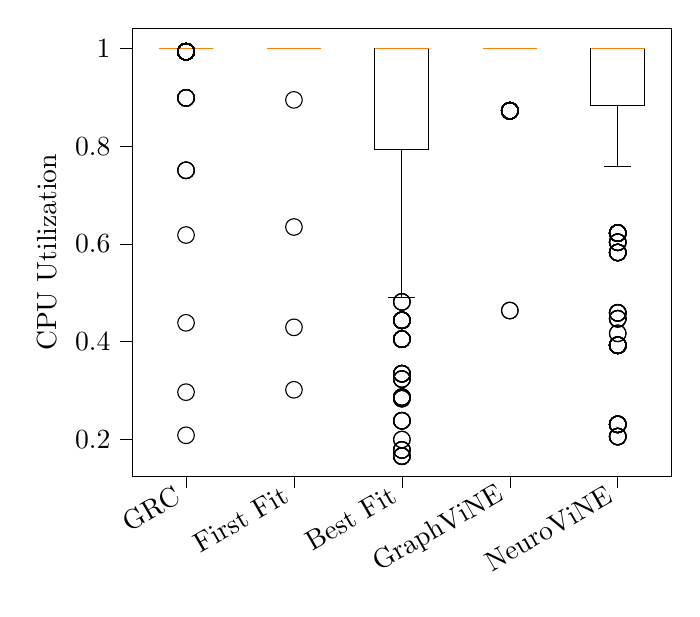
\begin{tikzpicture}

\definecolor{color0}{rgb}{1,0.498039215686275,0.0549019607843137}

\begin{axis}[
tick align=outside,
tick pos=left,
x grid style={white!69.0196078431373!black},
xmin=0.5, xmax=5.5,
xtick style={color=black},
xtick={1,2,3,4,5},
xticklabels={GRC,First Fit,Best Fit,GraphViNE,NeuroViNE},
y grid style={white!69.0196078431373!black},
ymin=0.123684210526316, ymax=1.04172932330827,
ytick style={color=black},
x tick label style={rotate=30,anchor=east},
ylabel={CPU Utilization},
]
\addplot [black]
table {%
0.75 1
1.25 1
1.25 1
0.75 1
0.75 1
};
\addplot [black]
table {%
1 1
1 1
};
\addplot [black]
table {%
1 1
1 1
};
\addplot [black]
table {%
0.875 1
1.125 1
};
\addplot [black]
table {%
0.875 1
1.125 1
};
\addplot [black, mark=*, mark size=3, mark options={solid,fill opacity=0}, only marks]
table {%
1 0.20820189274448
1 0.296529968454259
1 0.438485804416404
1 0.618296529968454
1 0.750788643533123
1 0.750788643533123
1 0.750788643533123
1 0.899053627760252
1 0.899053627760252
1 0.899053627760252
1 0.899053627760252
1 0.899053627760252
1 0.899053627760252
1 0.993690851735016
1 0.993690851735016
1 0.993690851735016
1 0.993690851735016
1 0.993690851735016
1 0.993690851735016
1 0.993690851735016
1 0.993690851735016
1 0.993690851735016
1 0.993690851735016
1 0.993690851735016
1 0.993690851735016
1 0.993690851735016
1 0.993690851735016
1 0.993690851735016
1 0.993690851735016
1 0.993690851735016
1 0.993690851735016
1 0.993690851735016
1 0.993690851735016
1 0.993690851735016
1 0.993690851735016
1 0.993690851735016
1 0.993690851735016
1 0.993690851735016
1 0.993690851735016
1 0.993690851735016
1 0.993690851735016
1 0.993690851735016
1 0.993690851735016
1 0.993690851735016
1 0.993690851735016
1 0.993690851735016
1 0.993690851735016
1 0.993690851735016
1 0.993690851735016
1 0.993690851735016
1 0.993690851735016
1 0.993690851735016
1 0.993690851735016
1 0.993690851735016
1 0.993690851735016
1 0.993690851735016
1 0.993690851735016
1 0.993690851735016
1 0.993690851735016
1 0.993690851735016
1 0.993690851735016
1 0.993690851735016
1 0.993690851735016
1 0.993690851735016
1 0.993690851735016
1 0.993690851735016
1 0.993690851735016
1 0.993690851735016
1 0.993690851735016
1 0.993690851735016
1 0.993690851735016
1 0.993690851735016
1 0.993690851735016
1 0.993690851735016
1 0.993690851735016
1 0.993690851735016
1 0.993690851735016
1 0.993690851735016
1 0.993690851735016
1 0.993690851735016
1 0.993690851735016
1 0.993690851735016
1 0.993690851735016
1 0.993690851735016
1 0.993690851735016
1 0.993690851735016
1 0.993690851735016
1 0.993690851735016
1 0.993690851735016
1 0.993690851735016
1 0.993690851735016
1 0.993690851735016
1 0.993690851735016
1 0.993690851735016
1 0.993690851735016
1 0.993690851735016
1 0.993690851735016
1 0.993690851735016
1 0.993690851735016
1 0.993690851735016
1 0.993690851735016
1 0.993690851735016
1 0.993690851735016
1 0.993690851735016
1 0.993690851735016
1 0.993690851735016
1 0.993690851735016
1 0.993690851735016
1 0.993690851735016
1 0.993690851735016
1 0.993690851735016
1 0.993690851735016
1 0.993690851735016
1 0.993690851735016
1 0.993690851735016
1 0.993690851735016
1 0.993690851735016
1 0.993690851735016
1 0.993690851735016
1 0.993690851735016
1 0.993690851735016
1 0.993690851735016
1 0.993690851735016
1 0.993690851735016
1 0.993690851735016
1 0.993690851735016
1 0.993690851735016
1 0.993690851735016
1 0.993690851735016
1 0.993690851735016
1 0.993690851735016
1 0.993690851735016
1 0.993690851735016
1 0.993690851735016
1 0.993690851735016
1 0.993690851735016
1 0.993690851735016
1 0.993690851735016
1 0.993690851735016
1 0.993690851735016
1 0.993690851735016
1 0.993690851735016
1 0.993690851735016
1 0.993690851735016
1 0.993690851735016
1 0.993690851735016
1 0.993690851735016
1 0.993690851735016
1 0.993690851735016
1 0.993690851735016
1 0.993690851735016
1 0.993690851735016
1 0.993690851735016
1 0.993690851735016
1 0.993690851735016
1 0.993690851735016
1 0.993690851735016
1 0.993690851735016
1 0.993690851735016
1 0.993690851735016
1 0.993690851735016
1 0.993690851735016
1 0.993690851735016
1 0.993690851735016
1 0.993690851735016
1 0.993690851735016
1 0.993690851735016
1 0.993690851735016
1 0.993690851735016
1 0.993690851735016
1 0.993690851735016
1 0.993690851735016
1 0.993690851735016
1 0.993690851735016
1 0.993690851735016
1 0.993690851735016
1 0.993690851735016
1 0.993690851735016
1 0.993690851735016
1 0.993690851735016
1 0.993690851735016
1 0.993690851735016
1 0.993690851735016
1 0.993690851735016
1 0.993690851735016
1 0.993690851735016
1 0.993690851735016
1 0.993690851735016
1 0.993690851735016
1 0.993690851735016
1 0.993690851735016
1 0.993690851735016
1 0.993690851735016
1 0.993690851735016
1 0.993690851735016
1 0.993690851735016
1 0.993690851735016
1 0.993690851735016
1 0.993690851735016
1 0.993690851735016
1 0.993690851735016
1 0.993690851735016
1 0.993690851735016
1 0.993690851735016
1 0.993690851735016
1 0.993690851735016
1 0.993690851735016
1 0.993690851735016
1 0.993690851735016
1 0.993690851735016
1 0.993690851735016
};
\addplot [black]
table {%
1.75 1
2.25 1
2.25 1
1.75 1
1.75 1
};
\addplot [black]
table {%
2 1
2 1
};
\addplot [black]
table {%
2 1
2 1
};
\addplot [black]
table {%
1.875 1
2.125 1
};
\addplot [black]
table {%
1.875 1
2.125 1
};
\addplot [black, mark=*, mark size=3, mark options={solid,fill opacity=0}, only marks]
table {%
2 0.301369863013699
2 0.429223744292237
2 0.634703196347032
2 0.894977168949772
};
\addplot [black]
table {%
2.75 0.793103448275862
3.25 0.793103448275862
3.25 1
2.75 1
2.75 0.793103448275862
};
\addplot [black]
table {%
3 0.793103448275862
3 0.490566037735849
};
\addplot [black]
table {%
3 1
3 1
};
\addplot [black]
table {%
2.875 0.490566037735849
3.125 0.490566037735849
};
\addplot [black]
table {%
2.875 1
3.125 1
};
\addplot [black, mark=*, mark size=3, mark options={solid,fill opacity=0}, only marks]
table {%
3 0.165413533834586
3 0.165413533834586
3 0.165413533834586
3 0.165413533834586
3 0.165413533834586
3 0.165413533834586
3 0.178191489361702
3 0.178191489361702
3 0.178191489361702
3 0.178191489361702
3 0.19949494949495
3 0.19949494949495
3 0.237974683544304
3 0.237974683544304
3 0.237974683544304
3 0.237974683544304
3 0.237974683544304
3 0.237974683544304
3 0.283208020050125
3 0.283208020050125
3 0.283208020050125
3 0.286096256684492
3 0.286096256684492
3 0.286096256684492
3 0.286096256684492
3 0.286096256684492
3 0.286096256684492
3 0.286096256684492
3 0.286096256684492
3 0.323232323232323
3 0.323232323232323
3 0.323232323232323
3 0.323232323232323
3 0.334231805929919
3 0.334231805929919
3 0.334231805929919
3 0.334231805929919
3 0.334231805929919
3 0.334231805929919
3 0.334231805929919
3 0.405063291139241
3 0.405063291139241
3 0.405063291139241
3 0.405063291139241
3 0.405063291139241
3 0.405063291139241
3 0.405063291139241
3 0.405063291139241
3 0.405063291139241
3 0.405063291139241
3 0.405063291139241
3 0.405063291139241
3 0.443609022556391
3 0.443609022556391
3 0.443609022556391
3 0.443609022556391
3 0.443609022556391
3 0.443609022556391
3 0.443609022556391
3 0.443609022556391
3 0.443609022556391
3 0.443609022556391
3 0.443609022556391
3 0.443609022556391
3 0.443609022556391
3 0.443609022556391
3 0.443609022556391
3 0.481283422459893
3 0.481283422459893
3 0.481283422459893
};
\addplot [black]
table {%
3.75 1
4.25 1
4.25 1
3.75 1
3.75 1
};
\addplot [black]
table {%
4 1
4 1
};
\addplot [black]
table {%
4 1
4 1
};
\addplot [black]
table {%
3.875 1
4.125 1
};
\addplot [black]
table {%
3.875 1
4.125 1
};
\addplot [black, mark=*, mark size=3, mark options={solid,fill opacity=0}, only marks]
table {%
4 0.463636363636364
4 0.463636363636364
4 0.872727272727273
4 0.872727272727273
4 0.872727272727273
4 0.872727272727273
4 0.872727272727273
4 0.872727272727273
4 0.872727272727273
4 0.872727272727273
4 0.872727272727273
4 0.872727272727273
4 0.872727272727273
4 0.872727272727273
4 0.872727272727273
4 0.872727272727273
4 0.872727272727273
4 0.872727272727273
4 0.872727272727273
4 0.872727272727273
4 0.872727272727273
4 0.872727272727273
4 0.872727272727273
4 0.872727272727273
4 0.872727272727273
4 0.872727272727273
4 0.872727272727273
4 0.872727272727273
4 0.872727272727273
4 0.872727272727273
4 0.872727272727273
4 0.872727272727273
4 0.872727272727273
4 0.872727272727273
4 0.872727272727273
4 0.872727272727273
4 0.872727272727273
4 0.872727272727273
4 0.872727272727273
4 0.872727272727273
4 0.872727272727273
4 0.872727272727273
4 0.872727272727273
4 0.872727272727273
4 0.872727272727273
};
\addplot [black]
table {%
4.75 0.883458646616541
5.25 0.883458646616541
5.25 1
4.75 1
4.75 0.883458646616541
};
\addplot [black]
table {%
5 0.883458646616541
5 0.759358288770054
};
\addplot [black]
table {%
5 1
5 1
};
\addplot [black]
table {%
4.875 0.759358288770054
5.125 0.759358288770054
};
\addplot [black]
table {%
4.875 1
5.125 1
};
\addplot [black, mark=*, mark size=3, mark options={solid,fill opacity=0}, only marks]
table {%
5 0.205607476635514
5 0.205607476635514
5 0.205607476635514
5 0.205607476635514
5 0.205607476635514
5 0.205607476635514
5 0.205607476635514
5 0.230576441102757
5 0.230576441102757
5 0.230576441102757
5 0.230576441102757
5 0.230576441102757
5 0.230576441102757
5 0.230576441102757
5 0.230576441102757
5 0.230576441102757
5 0.230576441102757
5 0.230576441102757
5 0.230576441102757
5 0.230576441102757
5 0.230576441102757
5 0.392523364485981
5 0.392523364485981
5 0.392523364485981
5 0.392523364485981
5 0.392523364485981
5 0.392523364485981
5 0.392523364485981
5 0.392523364485981
5 0.392523364485981
5 0.392523364485981
5 0.392523364485981
5 0.392523364485981
5 0.392523364485981
5 0.392523364485981
5 0.392523364485981
5 0.392523364485981
5 0.392523364485981
5 0.392523364485981
5 0.392523364485981
5 0.392523364485981
5 0.392523364485981
5 0.392523364485981
5 0.392523364485981
5 0.392523364485981
5 0.392523364485981
5 0.392523364485981
5 0.416938110749186
5 0.416938110749186
5 0.446808510638298
5 0.446808510638298
5 0.446808510638298
5 0.446808510638298
5 0.458923512747875
5 0.458923512747875
5 0.458923512747875
5 0.458923512747875
5 0.458923512747875
5 0.458923512747875
5 0.582554517133956
5 0.582554517133956
5 0.582554517133956
5 0.582554517133956
5 0.582554517133956
5 0.582554517133956
5 0.582554517133956
5 0.582554517133956
5 0.582554517133956
5 0.582554517133956
5 0.603448275862069
5 0.603448275862069
5 0.603448275862069
5 0.603448275862069
5 0.603448275862069
5 0.603448275862069
5 0.622149837133551
5 0.622149837133551
5 0.622149837133551
5 0.622149837133551
5 0.622149837133551
5 0.622149837133551
5 0.622149837133551
5 0.622149837133551
5 0.622149837133551
5 0.622149837133551
5 0.622149837133551
5 0.622149837133551
5 0.622149837133551
5 0.622149837133551
5 0.622149837133551
5 0.622149837133551
5 0.622149837133551
5 0.622149837133551
5 0.622149837133551
5 0.622149837133551
5 0.622149837133551
};
\addplot [color0]
table {%
0.75 1
1.25 1
};
\addplot [color0]
table {%
1.75 1
2.25 1
};
\addplot [color0]
table {%
2.75 1
3.25 1
};
\addplot [color0]
table {%
3.75 1
4.25 1
};
\addplot [color0]
table {%
4.75 1
5.25 1
};
\end{axis}

\end{tikzpicture}

  			}%
  			\caption{بهره‌وری \lr{CPU}}
  			\label{fig:bp-cpu-util}
  		\end{minipage}
  		\hfil
  		\begin{minipage}{.43\linewidth}
  			\centering
  			\resizebox{\linewidth}{!}{%
  				% This file was created by tikzplotlib v0.9.2.
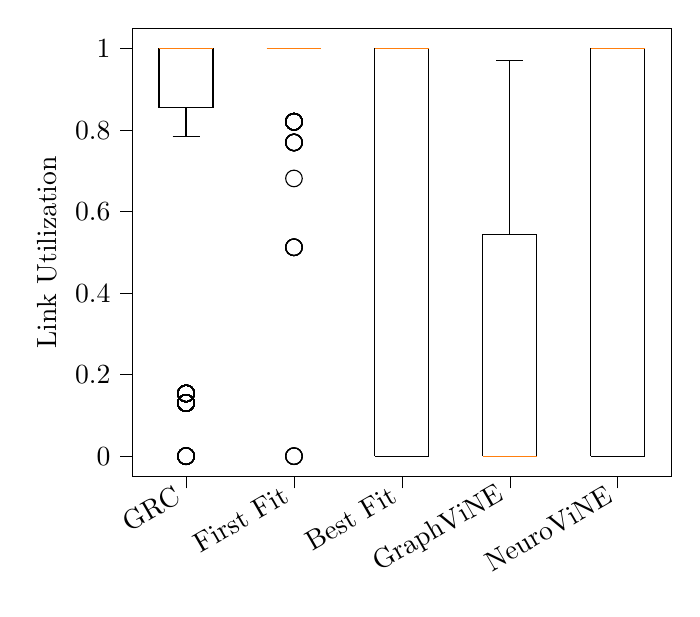
\begin{tikzpicture}

\definecolor{color0}{rgb}{1,0.498039215686275,0.0549019607843137}

\begin{axis}[
tick align=outside,
tick pos=left,
x grid style={white!69.0196078431373!black},
xmin=0.5, xmax=5.5,
xtick style={color=black},
xtick={1,2,3,4,5},
xticklabels={GRC,First Fit,Best Fit,GraphViNE,NeuroViNE},
y grid style={white!69.0196078431373!black},
ymin=-0.05, ymax=1.05,
ytick style={color=black},
x tick label style={rotate=30,anchor=east},
ylabel={Link Utilization},
]
\addplot [black]
table {%
0.75 0.855421686746988
1.25 0.855421686746988
1.25 1
0.75 1
0.75 0.855421686746988
};
\addplot [black]
table {%
1 0.855421686746988
1 0.78448275862069
};
\addplot [black]
table {%
1 1
1 1
};
\addplot [black]
table {%
0.875 0.78448275862069
1.125 0.78448275862069
};
\addplot [black]
table {%
0.875 1
1.125 1
};
\addplot [black, mark=*, mark size=3, mark options={solid,fill opacity=0}, only marks]
table {%
1 0
1 0
1 0
1 0
1 0
1 0
1 0
1 0
1 0
1 0
1 0
1 0
1 0
1 0.130434782608696
1 0.130434782608696
1 0.130434782608696
1 0.130434782608696
1 0.130434782608696
1 0.130434782608696
1 0.130434782608696
1 0.130434782608696
1 0.130434782608696
1 0.130434782608696
1 0.130434782608696
1 0.130434782608696
1 0.130434782608696
1 0.130434782608696
1 0.130434782608696
1 0.130434782608696
1 0.130434782608696
1 0.130434782608696
1 0.130434782608696
1 0.130434782608696
1 0.130434782608696
1 0.130434782608696
1 0.130434782608696
1 0.130434782608696
1 0.130434782608696
1 0.130434782608696
1 0.130434782608696
1 0.130434782608696
1 0.130434782608696
1 0.130434782608696
1 0.130434782608696
1 0.130434782608696
1 0.130434782608696
1 0.130434782608696
1 0.130434782608696
1 0.130434782608696
1 0.130434782608696
1 0.130434782608696
1 0.130434782608696
1 0.130434782608696
1 0.130434782608696
1 0.130434782608696
1 0.130434782608696
1 0.130434782608696
1 0.130434782608696
1 0.130434782608696
1 0.130434782608696
1 0.130434782608696
1 0.130434782608696
1 0.130434782608696
1 0.130434782608696
1 0.130434782608696
1 0.130434782608696
1 0.130434782608696
1 0.130434782608696
1 0.130434782608696
1 0.130434782608696
1 0.130434782608696
1 0.130434782608696
1 0.130434782608696
1 0.130434782608696
1 0.130434782608696
1 0.130434782608696
1 0.130434782608696
1 0.130434782608696
1 0.130434782608696
1 0.130434782608696
1 0.130434782608696
1 0.130434782608696
1 0.130434782608696
1 0.130434782608696
1 0.130434782608696
1 0.130434782608696
1 0.130434782608696
1 0.130434782608696
1 0.130434782608696
1 0.130434782608696
1 0.130434782608696
1 0.130434782608696
1 0.130434782608696
1 0.130434782608696
1 0.130434782608696
1 0.130434782608696
1 0.130434782608696
1 0.130434782608696
1 0.130434782608696
1 0.130434782608696
1 0.130434782608696
1 0.130434782608696
1 0.130434782608696
1 0.130434782608696
1 0.130434782608696
1 0.130434782608696
1 0.130434782608696
1 0.130434782608696
1 0.130434782608696
1 0.130434782608696
1 0.130434782608696
1 0.130434782608696
1 0.130434782608696
1 0.130434782608696
1 0.130434782608696
1 0.130434782608696
1 0.130434782608696
1 0.130434782608696
1 0.130434782608696
1 0.130434782608696
1 0.130434782608696
1 0.130434782608696
1 0.130434782608696
1 0.130434782608696
1 0.130434782608696
1 0.130434782608696
1 0.130434782608696
1 0.130434782608696
1 0.130434782608696
1 0.130434782608696
1 0.130434782608696
1 0.130434782608696
1 0.130434782608696
1 0.130434782608696
1 0.130434782608696
1 0.130434782608696
1 0.130434782608696
1 0.130434782608696
1 0.130434782608696
1 0.130434782608696
1 0.130434782608696
1 0.130434782608696
1 0.130434782608696
1 0.130434782608696
1 0.130434782608696
1 0.130434782608696
1 0.130434782608696
1 0.130434782608696
1 0.130434782608696
1 0.130434782608696
1 0.130434782608696
1 0.153846153846154
1 0.153846153846154
1 0.153846153846154
1 0.153846153846154
1 0.153846153846154
1 0.153846153846154
1 0.153846153846154
1 0.153846153846154
1 0.153846153846154
1 0.153846153846154
1 0.153846153846154
1 0.153846153846154
1 0.153846153846154
1 0.153846153846154
1 0.153846153846154
1 0.153846153846154
1 0.153846153846154
1 0.153846153846154
1 0.153846153846154
1 0.153846153846154
1 0.153846153846154
1 0.153846153846154
1 0.153846153846154
1 0.153846153846154
1 0.153846153846154
1 0.153846153846154
1 0.153846153846154
1 0.153846153846154
1 0.153846153846154
1 0.153846153846154
1 0.153846153846154
1 0.153846153846154
1 0.153846153846154
1 0.153846153846154
1 0.153846153846154
1 0.153846153846154
1 0.153846153846154
1 0.153846153846154
1 0.153846153846154
1 0.153846153846154
1 0.153846153846154
1 0.153846153846154
1 0.153846153846154
1 0.153846153846154
1 0.153846153846154
1 0.153846153846154
1 0.153846153846154
1 0.153846153846154
1 0.153846153846154
1 0.153846153846154
1 0.153846153846154
1 0.153846153846154
1 0.153846153846154
1 0.153846153846154
1 0.153846153846154
1 0.153846153846154
1 0.153846153846154
1 0.153846153846154
1 0.153846153846154
1 0.153846153846154
};
\addplot [black]
table {%
1.75 1
2.25 1
2.25 1
1.75 1
1.75 1
};
\addplot [black]
table {%
2 1
2 1
};
\addplot [black]
table {%
2 1
2 1
};
\addplot [black]
table {%
1.875 1
2.125 1
};
\addplot [black]
table {%
1.875 1
2.125 1
};
\addplot [black, mark=*, mark size=3, mark options={solid,fill opacity=0}, only marks]
table {%
2 0
2 0
2 0
2 0
2 0.5125
2 0.5125
2 0.5125
2 0.5125
2 0.5125
2 0.681388012618297
2 0.769716088328076
2 0.769716088328076
2 0.769716088328076
2 0.769716088328076
2 0.769716088328076
2 0.769716088328076
2 0.769716088328076
2 0.769716088328076
2 0.82051282051282
2 0.82051282051282
2 0.82051282051282
2 0.82051282051282
2 0.82051282051282
2 0.82051282051282
2 0.82051282051282
2 0.82051282051282
2 0.82051282051282
2 0.82051282051282
2 0.82051282051282
2 0.82051282051282
2 0.82051282051282
2 0.82051282051282
2 0.82051282051282
2 0.82051282051282
2 0.82051282051282
2 0.82051282051282
2 0.82051282051282
2 0.82051282051282
2 0.82051282051282
2 0.82051282051282
2 0.82051282051282
};
\addplot [black]
table {%
2.75 0
3.25 0
3.25 1
2.75 1
2.75 0
};
\addplot [black]
table {%
3 0
3 0
};
\addplot [black]
table {%
3 1
3 1
};
\addplot [black]
table {%
2.875 0
3.125 0
};
\addplot [black]
table {%
2.875 1
3.125 1
};
\addplot [black]
table {%
3.75 0
4.25 0
4.25 0.544943820224719
3.75 0.544943820224719
3.75 0
};
\addplot [black]
table {%
4 0
4 0
};
\addplot [black]
table {%
4 0.544943820224719
4 0.970588235294118
};
\addplot [black]
table {%
3.875 0
4.125 0
};
\addplot [black]
table {%
3.875 0.970588235294118
4.125 0.970588235294118
};
\addplot [black]
table {%
4.75 0
5.25 0
5.25 1
4.75 1
4.75 0
};
\addplot [black]
table {%
5 0
5 0
};
\addplot [black]
table {%
5 1
5 1
};
\addplot [black]
table {%
4.875 0
5.125 0
};
\addplot [black]
table {%
4.875 1
5.125 1
};
\addplot [color0]
table {%
0.75 1
1.25 1
};
\addplot [color0]
table {%
1.75 1
2.25 1
};
\addplot [color0]
table {%
2.75 1
3.25 1
};
\addplot [color0]
table {%
3.75 0
4.25 0
};
\addplot [color0]
table {%
4.75 1
5.25 1
};
\end{axis}

\end{tikzpicture}

  			}%
  			\caption{بهره‌وری لینک‌ها}
  			\label{fig:bp-link-util}
  		\end{minipage}
  		\hfill
  		\caption{بیشترین بهره‌وری از سرور‌ها و لینک‌ها در طول شبیه‌سازی}
  		\label{fig:max-util}
  	\end{figure}
  
  نمودارهای جعبه ای در شکل
   \ref {fig:max-util} 
   توزیع حداکثر بهره‌وری در استفاده از سرورها و پیوندها را در کل شبیه سازی نشان می‌دهد. شکل
   \ref {fig:bp-cpu-util} 
   نشان می‌دهد که \ourAlg\ سرورهای فعال با گره‌های مجازی را بسته بندی می‌کند و فقط تعداد کمی از سرورها را کم استفاده می‌کند. علاوه بر این‌، \ourAlg\ استفاده از پهنای باند را برای حفظ اتصال در سطح متوسط ​​نگه می‌دارد (نگاه کنید به شکل
    \ref {fig:bp-link-util})
    ). الگوریتم‌های \lr{Best Fit} و \lr{NeuroViNE} سطح بالایی از تعادل بار در استفاده از \lr{CPU} را برای حفظ توانایی تأمین نیازهای آینده نشان می‌دهند. با این حال‌، آنها عملکرد کمتری در استفاده از پهنای باند از خود نشان می‌دهند‌، که می‌تواند ناشی از عدم در نظر گرفتن همزمان سرورها و شبکه باشد. به همین ترتیب‌، روش‌های \lr{GRC} و\lr{ First Fit} دارای بهره‌وری سرور و پیوند بالایی هستند که توانایی آنها را برای نگاشت شبکه‌های مجازی محدود می‌کند.
    
    \subsection{\gls{arrival rate} شبکه مجازی}
    
    \begin{figure}[t]
    	% \vspace{0.05in}
    	\centering
    	\begin{minipage}{.3\linewidth}
    		\centering
    		\resizebox{\linewidth}{!}{%
    			
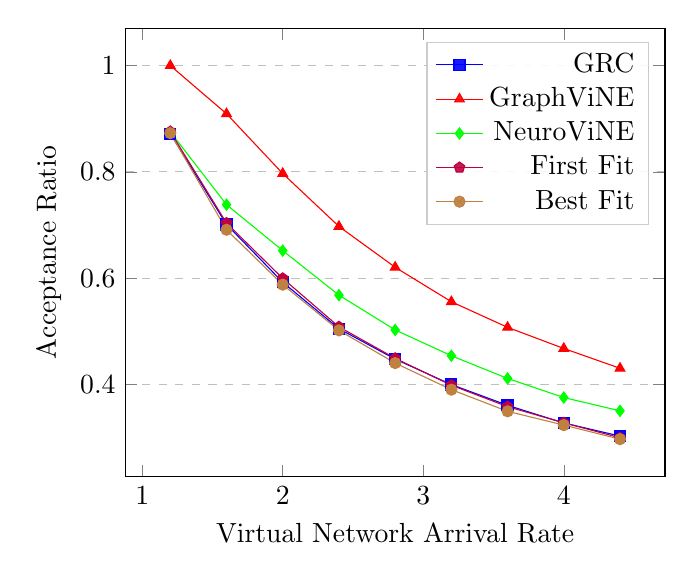
\begin{tikzpicture}
\begin{axis}[
    legend cell align={right},
    legend style={fill opacity=0.9, draw opacity=1, text opacity=1, draw=white!80!black},
    xlabel={Virtual Network Arrival Rate},
    ylabel={Acceptance Ratio},
    legend pos=north east,
    ymajorgrids=true,
    grid style=dashed,
]

\addplot[
    color=blue,
    mark=square*,
    ]
    coordinates {
(1.2,0.8720300125052105)
(1.6,0.7011566114410753)
(2.0,0.5923980995248812)
(2.4,0.5050020842017507)
(2.8,0.44783851375491246)
(3.2,0.39987494137877133)
(3.6,0.3608447964429623)
(4.0,0.3276228585719645)
(4.4,0.30297862664847663)
    };
\addlegendentry{GRC}

\addplot[
    color=red,
    mark=triangle*,
    ]
    coordinates {
(1.2,1.0)
(1.6,0.9093466708346358)
(2.0,0.7969492373093273)
(2.4,0.6973739057940809)
(2.8,0.6205787781350482)
(3.2,0.5557292480850399)
(3.6,0.507572599694317)
(4.0,0.46780042515943476)
(4.4,0.4305366075488859)
    };
\addlegendentry{GraphViNE}

\addplot[
    color=green,
    mark=diamond*,
    ]
    coordinates {
(1.2,0.8753647353063777)
(1.6,0.7383557361675523)
(2.0,0.6519129782445612)
(2.4,0.5681533972488537)
(2.8,0.502679528403001)
(3.2,0.45411911833672036)
(3.6,0.4114214255939975)
(4.0,0.37551581843191195)
(4.4,0.35050022737608)
    };
\addlegendentry{NeuroViNE}

\addplot[
    color=purple,
    mark=pentagon*,
    ]
    coordinates {
(1.2,0.8757815756565236)
(1.6,0.7036573929352923)
(2.0,0.5996499124781196)
(2.4,0.5085452271779909)
(2.8,0.4492675955698464)
(3.2,0.3986243551664843)
(3.6,0.358343754342087)
(4.0,0.3279979992497186)
(4.4,0.29979536152796726)
    };
\addlegendentry{First Fit}

\addplot[
    color=brown,
    mark=otimes*,
    ]
    coordinates {
(1.2,0.8728636932055023)
(1.6,0.6911534854642076)
(2.0,0.5878969742435609)
(2.4,0.5018757815756565)
(2.8,0.44033583422650946)
(3.2,0.3903392215100828)
(3.6,0.34959010698902315)
(4.0,0.3236213580092535)
(4.4,0.29718053660754884)
    };
\addlegendentry{Best Fit}





\end{axis}
\end{tikzpicture}


    		}%
    		\caption{نرخ پذیرش}
    		\label{fig:diff-load-ar}
    	\end{minipage}
    	\hfil
    	\begin{minipage}{.3\linewidth}
    		\centering
    		\resizebox{\linewidth}{!}{%
    			
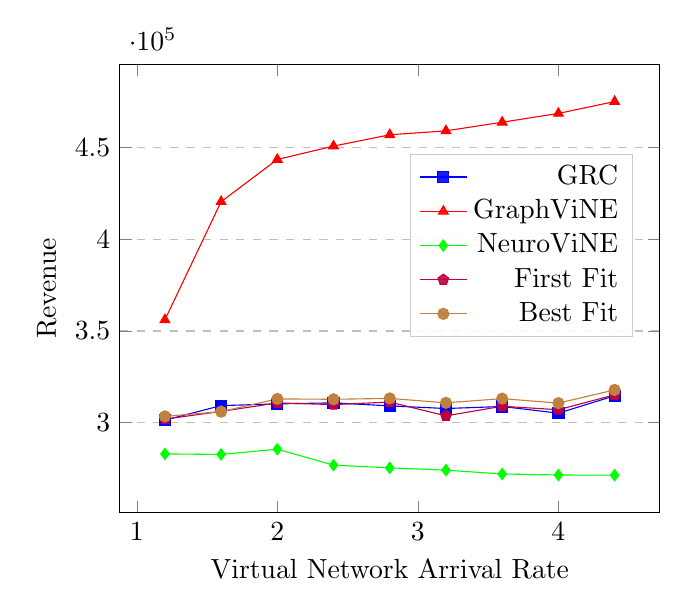
\begin{tikzpicture}
\begin{axis}[
    legend cell align={right},
    legend style={fill opacity=0.9, draw opacity=1, text opacity=1, draw=white!80!black, at={(0.95,0.8)}},
    xlabel={Virtual Network Arrival Rate},
    ylabel={Revenue},
    % xmin=0, xmax=100  ,
    % ymin=0, ymax=1,
    % xtick={0,10,30,50,70,90, 100},
    % ytick={0,100,200,300,400,500},
    % legend pos=north east,
    ymajorgrids=true,
    grid style=dashed,
]

\addplot[
    color=blue,
    mark=square*,
    ]
    coordinates {
(1.2,301420)
(1.6,309334)
(2.0,310278)
(2.4,310838)
(2.8,309192)
(3.2,307755)
(3.6,308847)
(4.0,305227)
(4.4,314684)
    };
\addlegendentry{GRC}

\addplot[
    color=red,
    mark=triangle*,
    ]
    coordinates {
(1.2,356068)
(1.6,420413)
(2.0,443410)
(2.4,450674)
(2.8,456853)
(3.2,458993)
(3.6,463679)
(4.0,468482)
(4.4,474940)
    };
\addlegendentry{GraphViNE}

\addplot[
    color=green,
    mark=diamond*,
    ]
    coordinates {
(1.2,283022)
(1.6,282743)
(2.0,285606)
(2.4,276905)
(2.8,275439)
(3.2,274172)
(3.6,272108)
(4.0,271536)
(4.4,271459)
    };
\addlegendentry{NeuroViNE}

\addplot[
    color=purple,
    mark=pentagon*,
    ]
    coordinates {
(1.2,301981)
(1.6,306181)
(2.0,310806)
(2.4,309881)
(2.8,311278)
(3.2,303764)
(3.6,308979)
(4.0,307101)
(4.4,315203)
    };
\addlegendentry{First Fit}

\addplot[
    color=brown,
    mark=otimes*,
    ]
    coordinates {
(1.2,303472)
(1.6,306062)
(2.0,312989)
(2.4,312785)
(2.8,313259)
(3.2,310856)
(3.6,313145)
(4.0,310685)
(4.4,317893)
    };
\addlegendentry{Best Fit}






\end{axis}
\end{tikzpicture}
    		}%
    		\caption{درآمد}
    		\label{fig:diff-load-rev}
    	\end{minipage} 
    	\begin{minipage}{.3\linewidth}
    		\centering
    		\resizebox{\linewidth}{!}{%
    			
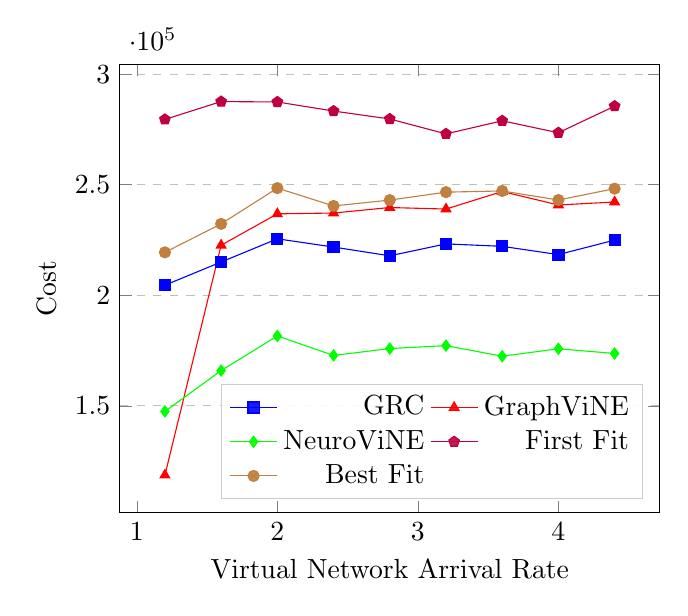
\begin{tikzpicture}
\begin{axis}[
    legend cell align={right},
    legend style={fill opacity=0.9, draw opacity=1, text opacity=1, draw=white!80!black, legend columns=2},
    xlabel={Virtual Network Arrival Rate},
    ylabel={Cost},
    % xmin=0, xmax=100  ,
    % ymin=0, ymax=1,
    % xtick={0,10,30,50,70,90, 100},
    % ytick={0,100,200,300,400,500},
    legend pos=south east,
    ymajorgrids=true,
    grid style=dashed,
]

\addplot[
    color=blue,
    mark=square*,
    ]
    coordinates {
(1.2,204590)
(1.6,215062)
(2.0,225549)
(2.4,221827)
(2.8,217870)
(3.2,223254)
(3.6,222156)
(4.0,218417)
(4.4,224980)
    };
\addlegendentry{GRC}

\addplot[
    color=red,
    mark=triangle*,
    ]
    coordinates {
(1.2,118709)
(1.6,222658)
(2.0,236842)
(2.4,237209)
(2.8,239696)
(3.2,239006)
(3.6,246934)
(4.0,240842)
(4.4,242192)
    };
\addlegendentry{GraphViNE}

\addplot[
    color=green,
    mark=diamond*,
    ]
    coordinates {
(1.2,147528)
(1.6,165987)
(2.0,181638)
(2.4,172834)
(2.8,175939)
(3.2,177263)
(3.6,172484)
(4.0,175840)
(4.4,173720)
    };
\addlegendentry{NeuroViNE}

\addplot[
    color=purple,
    mark=pentagon*,
    ]
    coordinates {
(1.2,279525)
(1.6,287596)
(2.0,287405)
(2.4,283311)
(2.8,279715)
(3.2,272984)
(3.6,278894)
(4.0,273495)
(4.4,285522)
    };
\addlegendentry{First Fit}

\addplot[
    color=brown,
    mark=otimes*,
    ]
    coordinates {
(1.2,219426)
(1.6,232311)
(2.0,248473)
(2.4,240412)
(2.8,243051)
(3.2,246649)
(3.6,247187)
(4.0,243090)
(4.4,248232)
    };
\addlegendentry{Best Fit}







\end{axis}
\end{tikzpicture}

    		}%
    		\caption{هزینه}
    		\label{fig:diff-load-cost}
    	\end{minipage}
    	\caption{مقایسه معیارها با نرخ‌های ورود شبکه‌ مجازی متفاوت}
    	\label{fig:diff-load}
    \end{figure}
    
    برای اندازه گیری بیشتر مقیاس پذیری و عملکرد‌، ما \ourAlg\ را با الگوریتم‌های دیگر تحت نرخ‌های مختلف ورود شبکه مجازی (یعنی بار‌های مختلف) مقایسه کردیم. به طور خاص‌، ما نرخ‌های مختلف ورود را بین $ 1.2 $ و $ 4.4 $ بررسی کردیم  و نتایج را در شکل  \ref{fig:diff-load}  ارائه دادیم.
    از شکل \ref{fig:diff-load-ar} مشهود است که با افزایش نرخ ورود‌، میزان پذیرش درخواست‌ها کاهش می‌یابد. با این وجود‌، میزان قبولی حاصل از \ourAlg\ در مقایسه با الگوریتم‌های دیگر به طور مداوم بالاتر است. مشاهده می‌کنیم که \lr{NeuroViNE} مقیاس پذیری بهتری از خود نشان می‌دهد‌، اما عملکرد آن هنوز حدود 18 درصد کمتر از روش ما است. \lr{NeuroViNE} درآمد و هزینه کمی دارد که نشان می‌دهد نسبت پذیرش بالاتر آن از توانایی آن در جاسازی \lr{VN}‌های کوچکتر ناشی می‌شود که درآمد کمتری دارند.
     اگرچه نرخ پذیرش درخواست‌ها کاهش می‌یابد‌، اما \ourAlg\ موفق می‌شود تعداد شبکه‌های مجازی تعبیه شده را افزایش دهد که منجر به درآمد و هزینه بالاتر می‌شود (به شکل \ref{fig:diff-load-rev} و \ref{fig:diff-load-cost} نگاه کنید). با این حال‌، الگوریتم‌های دیگر در محدودیت $ 2 $ شبکه مجازی در هر واحد از زمان هستند‌، و در نتیجه درآمد و هزینه آنها تغییر قابل توجهی نمی‌کند.
     
      \subsection{تقاضای منبع پیوند مجازی}
      
      \begin{figure*}[t]
      	\centering
      	% \vspace{0.03in}
      	\begin{minipage}{.29\linewidth}
      		\centering
      		\resizebox{\linewidth}{!}{%
      			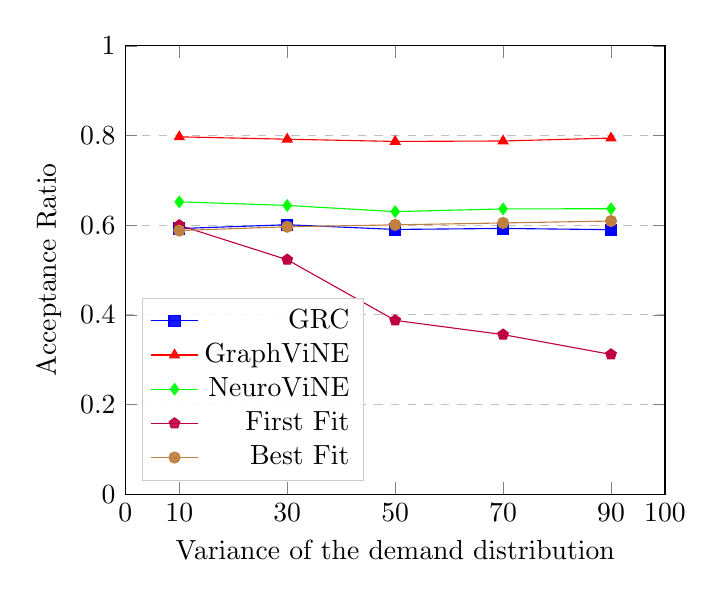
\begin{tikzpicture}
\begin{axis}[
    legend cell align={right},
    legend style={fill opacity=0.9, draw opacity=1, text opacity=1, draw=white!80!black},
    xlabel={Variance of the demand distribution},
    ylabel={Acceptance Ratio},
    xmin=0, xmax=100,
    ymin=0, ymax=1,
    xtick={0,10,30,50,70,90, 100},
    % ytick={0,100,200,300,400,500},
    legend pos=south west,
    ymajorgrids=true,
    grid style=dashed,
]

\addplot[
    color=blue,
    mark=square*,
    ]
    coordinates {
    (10,0.5923980995248812)
    (30,0.6009002250562641)
    (50,0.59039759939985)
    (70,0.5926481620405102)
    (90,0.5898974743685921)
    };
\addlegendentry{GRC}

\addplot[
    color=red,
    mark=triangle*,
    ]
    coordinates {
    (10,0.7969492373093273)
    (30,0.7916979244811203)
    (50,0.7866966741685422)
    (70,0.7876969242310577)
    (90,0.7941985496374093)
    };
\addlegendentry{GraphViNE}

\addplot[
    color=green,
    mark=diamond*,
    ]
    coordinates {
    (10,0.6519129782445612)
    (30,0.6439109777444361)
    (50,0.6301575393848462)
    (70,0.6361590397599399)
    (90,0.6366591647911978)
    };
\addlegendentry{NeuroViNE}

\addplot[
    color=purple,
    mark=pentagon*,
    ]
    coordinates {
(10,0.5996499124781196)
(30,0.5228807201800449)
(50,0.3875968992248062)
(70,0.35583895973993496)
(90,0.3115778944736184)
    };
\addlegendentry{First Fit}

\addplot[
    color=brown,
    mark=otimes*,
    ]
    coordinates {
(10,0.5878969742435609)
(30,0.5963990997749438)
(50,0.6006501625406351)
(70,0.6049012253063266)
(90,0.6091522880720179)
    };
\addlegendentry{Best Fit}





\end{axis}
\end{tikzpicture}
      		}%
      		\caption{نرخ پذیرش}
      		\label{fig:diff-link-ar}
      	\end{minipage}
      	\hfil
      	\begin{minipage}{.29\linewidth}
      		\centering
      		\resizebox{\linewidth}{!}{%
      			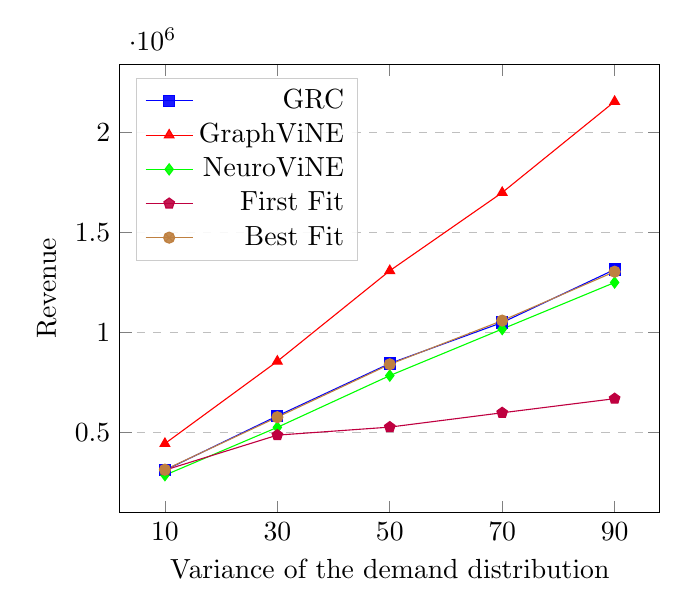
\begin{tikzpicture}
\begin{axis}[
    legend cell align={right},
    legend style={fill opacity=0.9, draw opacity=1, text opacity=1, draw=white!80!black},
    xlabel={Variance of the demand distribution},
    ylabel={Revenue},
    % xmin=0, xmax=100,
    % ymin=0, ymax=1,
    xtick={0,10,30,50,70,90, 100},
    % ytick={0,100,200,300,400,500},
    legend pos=north west,
    ymajorgrids=true,
    grid style=dashed,
]

\addplot[
    color=blue,
    mark=square*,
    ]
    coordinates {
(10,310278)
(30,581754)
(50,844107)
(70,1048861)
(90,1313781)
    };
\addlegendentry{GRC}

\addplot[
    color=red,
    mark=triangle*,
    ]
    coordinates {
(10,443410)
(30,854997)
(50,1307757)
(70,1698651)
(90,2153743)
    };
\addlegendentry{GraphViNE}

\addplot[
    color=green,
    mark=diamond*,
    ]
    coordinates {
(10,285606)
(30,524704)
(50,783399)
(70,1016251)
(90,1248881)
    };
\addlegendentry{NeuroViNE}

\addplot[
    color=purple,
    mark=pentagon*,
    ]
    coordinates {
(10,310806)
(30,485756)
(50,525896)
(70,597567)
(90,668085)
    };
\addlegendentry{First Fit}

\addplot[
    color=brown,
    mark=otimes*,
    ]
    coordinates {
(10,312989)
(30,575444)
(50,839820)
(70,1058408)
(90,1302955)
    };
\addlegendentry{Best Fit}





\end{axis}
\end{tikzpicture}
      		}%
      		\caption{درآمد}
      		\label{fig:diff-link-rev}
      	\end{minipage}
      	\hfil
      	\begin{minipage}{.29\linewidth}
      		\centering
      		\resizebox{\linewidth}{!}{%
      			
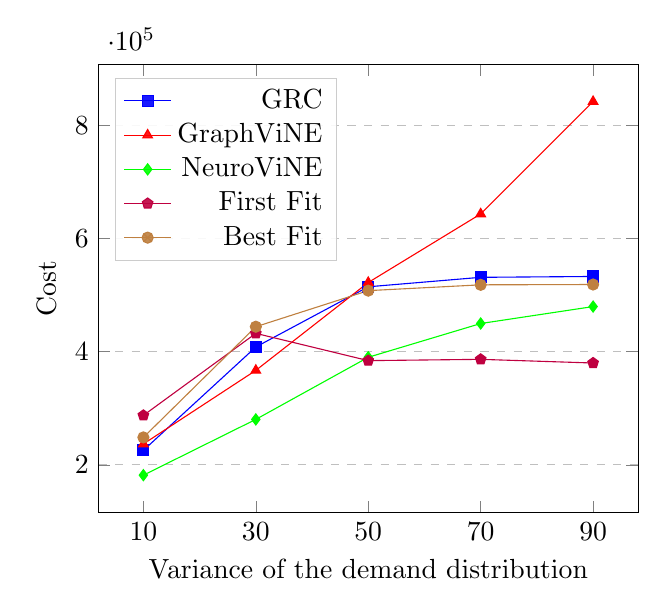
\begin{tikzpicture}
\begin{axis}[
    legend cell align={right},
    legend style={fill opacity=0.9, draw opacity=1, text opacity=1, draw=white!80!black},
    xlabel={Variance of the demand distribution},
    ylabel={Cost},
    % xmin=0, xmax=100,
    % ymin=0, ymax=1,
    xtick={0,10,30,50,70,90, 100},
    % ytick={0,100,200,300,400,500},
    legend pos=north west,
    ymajorgrids=true,
    grid style=dashed,
]

\addplot[
    color=blue,
    mark=square*,
    ]
    coordinates {
(10,225549)
(30,408456)
(50,514992)
(70,531753)
(90,533247)
    };
\addlegendentry{GRC}

\addplot[
    color=red,
    mark=triangle*,
    ]
    coordinates {
(10,236842)
(30,367070)
(50,522564)
(70,643883)
(90,842784)
    };
\addlegendentry{GraphViNE}

\addplot[
    color=green,
    mark=diamond*,
    ]
    coordinates {
(10,181638)
(30,280335)
(50,390260)
(70,449987)
(90,479996)
    };
\addlegendentry{NeuroViNE}

\addplot[
    color=purple,
    mark=pentagon*,
    ]
    coordinates {
(10,287405)
(30,432565)
(50,384316)
(70,386606)
(90,380101)
    };
\addlegendentry{First Fit}

\addplot[
    color=brown,
    mark=otimes*,
    ]
    coordinates {
(10,248473)
(30,444340)
(50,508184)
(70,518467)
(90,519020)
    };
\addlegendentry{Best Fit}





\end{axis}
\end{tikzpicture}
      		}%
      		\caption{هزینه}
      		\label{fig:diff-link-cost}
      	\end{minipage}
      	\caption{تاثیر تقاضاهای مختلف پیوند‌ مجازی}
      	\label{fig:diff-link}
      \end{figure*}
  
  در این آزمایش‌، ما تأثیر تقاضاهای  مختلف پیوند مجازی را بر عملکرد الگوریتم‌های مختلف بررسی می‌کنیم. بنابراین‌، ما واریانس درخواست‌های پیوند مجازی را که توزیعی نرمال با میانگین 4  است‌، از 10  به 90  تغییر می‌دهیم و نتایج را در شکل \ref{fig:diff-link} ارائه می‌دهیم.
  مشاهده می‌کنیم که \ourAlg\ قادر به نگاشت پیوندهای مجازی گسترده تر در سرورهای فیزیکی است و بنابراین نسبت پذیرش آن تغییر نمی‌کند که منجر به افزایش درآمد می‌شود (نگاه کنید به شکل \ref{fig:diff-link-rev} ). این روند برای الگوریتم های \lr{NeuroViNE}‌،\lr{ Best Fit} و \lr{GRC} نیز اتفاق می‌افتد‌، که نشان می‌دهد آنها نیز به اهمیت نگاشت پیوندهای مجازی بزرگ در داخل سرورهای فیزیکی آگاه هستند. با این حال‌، الگوریتم \lr{Firs Fit} از تقاضای پیوند مجازی بالا رنج می‌برد‌، که به طور قابل توجهی نسبت پذیرش آن را کاهش می‌دهد.
  \subsection{منابع چند‌بعدی}
  
      \begin{figure*}[t]
      	\centering
      	\begin{minipage}{.3\linewidth}
      		\centering
      		\resizebox{\linewidth}{!}{%
      			% This file was created by tikzplotlib v0.9.2.
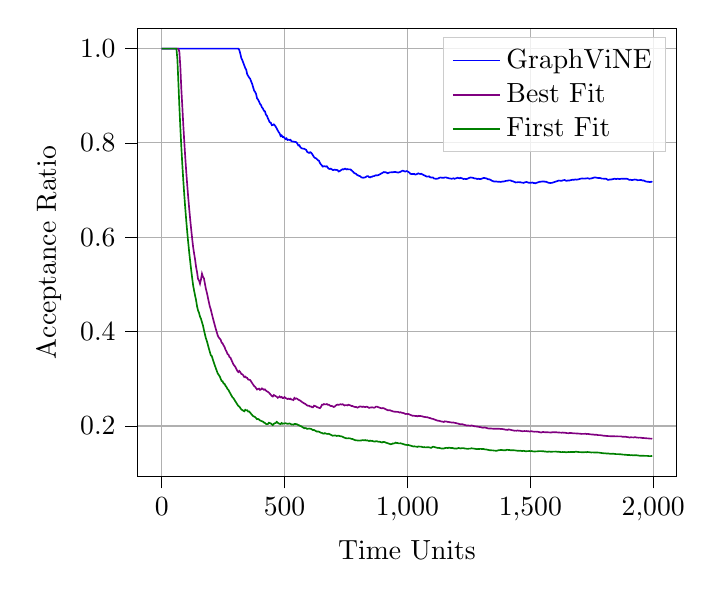
\begin{tikzpicture}

\definecolor{color0}{rgb}{0.501960784313725,0,0.501960784313725}

\begin{axis}[
legend cell align={left},
legend style={fill opacity=0.8, draw opacity=1, text opacity=1, draw=white!80!black},
tick align=outside,
tick pos=left,
x grid style={white!69.0196078431373!black},
xlabel={Time Units},
xmin=-99.8, xmax=2095.8,
xtick style={color=black},
y grid style={white!69.0196078431373!black},
ylabel={Acceptance Ratio},
ymin=0.0927620005026389, ymax=1.04320180949987,
ytick style={color=black},
ytick={0,0.2,0.4,0.6,0.8,1,1.2},
yticklabels={0.0,0.2,0.4,0.6,0.8,1.0,1.2},
ymajorgrids=true,
xmajorgrids=true,
]
\addplot [semithick, blue]
table {%
0 1
4 1
8 1
12 1
16 1
20 1
24 1
28 1
32 1
36 1
40 1
44 1
48 1
52 1
56 1
60 1
64 1
68 1
72 1
76 1
80 1
84 1
88 1
92 1
96 1
100 1
104 1
108 1
112 1
116 1
120 1
124 1
128 1
132 1
136 1
140 1
144 1
148 1
152 1
156 1
160 1
164 1
168 1
172 1
176 1
180 1
184 1
188 1
192 1
196 1
200 1
204 1
208 1
212 1
216 1
220 1
224 1
228 1
232 1
236 1
240 1
244 1
248 1
252 1
256 1
260 1
264 1
268 1
272 1
276 1
280 1
284 1
288 1
292 1
296 1
300 1
304 1
308 1
312 1
316 0.996850393700787
320 0.989113530326594
324 0.980030721966206
328 0.975720789074355
332 0.970014992503748
336 0.964444444444444
340 0.95900439238653
344 0.955137481910275
348 0.945636623748212
352 0.942008486562942
356 0.938461538461538
360 0.936376210235131
364 0.930232558139535
368 0.925575101488498
372 0.918340026773762
376 0.911258278145695
380 0.908256880733945
384 0.90402075226978
388 0.894736842105263
392 0.891994917407878
396 0.888050314465409
400 0.88293897882939
404 0.88039457459926
408 0.875457875457875
412 0.873035066505441
416 0.868263473053892
420 0.867141162514828
424 0.860164512338425
428 0.857974388824214
432 0.852364475201845
436 0.848
440 0.843714609286523
444 0.84287317620651
448 0.837597330367075
452 0.837927232635061
456 0.839344262295082
460 0.837486457204767
464 0.834586466165414
468 0.830670926517572
472 0.826821541710665
476 0.82303664921466
480 0.820353063343717
484 0.814624098867147
488 0.816138917262513
492 0.812563323201621
496 0.813065326633166
500 0.810568295114656
504 0.80811078140455
508 0.809617271835132
512 0.806231742940604
516 0.806763285024155
520 0.806327900287632
524 0.806850618458611
528 0.803588290840415
532 0.803186504217432
536 0.802790697674419
540 0.802400738688827
544 0.802016498625115
548 0.801637852593267
552 0.798554652213189
556 0.794618834080717
560 0.795191451469279
564 0.791335101679929
568 0.789288849868305
572 0.788142981691369
576 0.787878787878788
580 0.787618228718831
584 0.786507258753202
588 0.785411365564037
592 0.780960404380792
596 0.779916317991632
600 0.778886118038238
604 0.780346820809249
608 0.779327317473339
612 0.776691116544417
616 0.773279352226721
620 0.769911504424779
624 0.768185451638689
628 0.767275615567911
632 0.765588003157064
636 0.763137254901961
640 0.762275915822291
644 0.757552285050349
648 0.754426481909161
652 0.752104055087988
656 0.749809885931559
660 0.750566893424036
664 0.750563486100676
668 0.749813293502614
672 0.750556792873051
676 0.74760147601476
680 0.745414526779164
684 0.74471188913202
688 0.745467730239304
692 0.744051910598414
696 0.742652329749104
700 0.742694226657163
704 0.743444365698086
708 0.74277660324172
712 0.74281709880869
716 0.742160278745645
720 0.739431739431739
724 0.740179186767746
728 0.741603838245374
732 0.743012951601909
736 0.744406779661017
740 0.743762643290627
744 0.745137491616365
748 0.745163442294863
752 0.74386197743862
756 0.744554455445545
760 0.74392646093237
764 0.743958197256695
768 0.743989603638726
772 0.742081447963801
776 0.740192926045016
780 0.738323736404351
784 0.735837046467218
788 0.735275490816973
792 0.73408947700063
796 0.73166144200627
800 0.731129132875858
804 0.729981378026071
808 0.72946263125386
812 0.727105101413645
816 0.726605504587156
820 0.726110772976263
824 0.726832222895215
828 0.726943942133816
832 0.728254349130174
836 0.72955223880597
840 0.729649435531788
844 0.727380248373743
848 0.726898175397293
852 0.728178090216755
856 0.728279883381924
860 0.729541497388276
864 0.729636048526863
868 0.730879815986199
872 0.731539782484259
876 0.731054131054131
880 0.731707317073171
884 0.732354601919819
888 0.733558178752108
892 0.734750979294908
896 0.735933147632312
900 0.737104825291181
904 0.738266151297626
908 0.737768004398021
912 0.737821565407772
916 0.736784741144414
920 0.735756918068367
924 0.736898973527823
928 0.737493275954814
932 0.737546866630959
936 0.738133333333333
940 0.7376526818906
944 0.738233738762559
948 0.738283307003686
952 0.738332459360252
956 0.737859007832898
960 0.737389495579823
964 0.737441740031072
968 0.738009283135637
972 0.739085772984078
976 0.740153452685422
980 0.741212429954152
984 0.740740740740741
988 0.739767559373421
992 0.739305485656769
996 0.740350877192983
1000 0.739890164752871
1004 0.73843858776728
1008 0.736998514115899
1012 0.734583127775037
1016 0.734152334152334
1020 0.734214390602056
1024 0.734275962944905
1028 0.734337056823701
1032 0.732946298984035
1036 0.733493975903615
1040 0.734517522803649
1044 0.735533237685318
1048 0.734635540733683
1052 0.73421926910299
1056 0.734751773049645
1060 0.733396137541215
1064 0.732519943688409
1068 0.731182795698925
1072 0.730787144853284
1076 0.729002320185615
1080 0.728617660656496
1084 0.728696453247351
1088 0.729233593391464
1092 0.72748056698674
1096 0.726651480637813
1100 0.726736268724467
1104 0.726820443238354
1108 0.724650743578188
1112 0.724292770543332
1116 0.723937360178971
1120 0.724030316540348
1124 0.724566859173701
1128 0.725542275343072
1132 0.72651080723423
1136 0.726593406593407
1140 0.726237406920718
1144 0.726320384111742
1148 0.725967812092214
1152 0.726918075422627
1156 0.726997840172786
1160 0.726216099870857
1164 0.725868725868726
1168 0.725096194955109
1172 0.724755006391138
1176 0.724416135881104
1180 0.724079559881507
1184 0.724588781105019
1188 0.725094577553594
1192 0.723921240050272
1196 0.724843423799582
1200 0.725343320848939
1204 0.726254666113646
1208 0.725506407606449
1212 0.725175113308612
1216 0.726078028747433
1220 0.725337699549734
1224 0.724602203182375
1228 0.723464823098821
1232 0.723956222132144
1236 0.723636363636364
1240 0.723318566250504
1244 0.724207145724609
1248 0.725090036014406
1252 0.725967291583566
1256 0.726838966202783
1260 0.726516052318668
1264 0.726195179770842
1268 0.72587632926349
1272 0.724774244208873
1276 0.724853228962818
1280 0.724151385095591
1284 0.723453908984831
1288 0.724311748739822
1292 0.723618090452261
1296 0.723314065510597
1300 0.723780253553592
1304 0.724626579854462
1308 0.725467735777014
1312 0.725923106204796
1316 0.725237191650854
1320 0.724933787362845
1324 0.724254998113919
1328 0.722828130876269
1332 0.722909636295463
1336 0.722242990654206
1340 0.721207603428997
1344 0.719806763285024
1348 0.719155242682475
1352 0.718138160325083
1356 0.718232044198895
1360 0.718325376423063
1364 0.718051995606005
1368 0.717780211756115
1372 0.717874044412086
1376 0.717604355716878
1380 0.71733622873688
1384 0.717791411042945
1388 0.718243972652033
1392 0.718335127377108
1396 0.718783542039356
1400 0.719586157688191
1404 0.719672714336535
1408 0.720113515431004
1412 0.720551821719137
1416 0.720634920634921
1420 0.720365810763278
1424 0.719396702911259
1428 0.718782791185729
1432 0.718172305545867
1436 0.717217391304348
1440 0.716267776621575
1444 0.716361120719474
1448 0.716798896171093
1452 0.716890264877881
1456 0.71663807890223
1460 0.716729387615464
1464 0.715796656431252
1468 0.715889758421232
1472 0.71530369867662
1476 0.716074450084602
1480 0.716841039487006
1484 0.717266913497139
1488 0.716683450822424
1492 0.715768329427519
1496 0.715525876460768
1500 0.715617715617716
1504 0.715709066755231
1508 0.716131169261345
1512 0.715229600264288
1516 0.71499176276771
1520 0.714426552744003
1524 0.715175352343494
1528 0.715920235371036
1532 0.716661232474731
1536 0.71739837398374
1540 0.717807330522219
1544 0.717890650274992
1548 0.718296224588577
1552 0.71837785645317
1556 0.718459069020867
1560 0.717579250720461
1564 0.717981475566912
1568 0.716788786237655
1572 0.715919923736892
1576 0.715372424722662
1580 0.715143850774581
1584 0.71523178807947
1588 0.715319282793331
1592 0.716033887668654
1596 0.716744913928013
1600 0.717452388385888
1604 0.718156337589536
1608 0.718856787822305
1612 0.71955376510691
1616 0.720247295208655
1620 0.720012334258403
1624 0.719778529683174
1628 0.719852715556919
1632 0.720538720538721
1636 0.721221374045802
1640 0.721291501675297
1644 0.720145852324521
1648 0.719612003637466
1652 0.720290293317206
1656 0.720361990950226
1660 0.72043334336443
1664 0.721104773341339
1668 0.721473495058401
1672 0.722139229160442
1676 0.721609538002981
1680 0.722271781147785
1684 0.722634233165233
1688 0.722107132287659
1692 0.722468260997933
1696 0.722827687776141
1700 0.723479282985601
1704 0.724127821753151
1708 0.724480842351565
1712 0.724832214765101
1716 0.724308588064047
1720 0.724368283473715
1724 0.724717473196175
1728 0.724775946805435
1732 0.725122584366888
1736 0.724892086330935
1740 0.724088429514786
1744 0.724434259524491
1748 0.724778508145184
1752 0.725406330196749
1756 0.726031294452347
1760 0.726653420380358
1764 0.726989521382045
1768 0.72647640576434
1772 0.725965604736397
1776 0.725738396624473
1780 0.725792871175975
1784 0.725567068048166
1788 0.724783459066778
1792 0.724282129913577
1796 0.724339360222531
1800 0.724118789897308
1804 0.723899196898366
1808 0.72395689416966
1812 0.722911497105045
1816 0.721595598349381
1820 0.721932473236344
1824 0.722541769378253
1828 0.722328505056026
1832 0.722934278701936
1836 0.723265306122449
1840 0.723866413250068
1844 0.724193985369818
1848 0.723438767234388
1852 0.723765848394929
1856 0.724091520861373
1860 0.723609991941982
1864 0.723398552666845
1868 0.723990371757154
1872 0.724312783560181
1876 0.72410119840213
1880 0.724156258304544
1884 0.723945902943516
1888 0.72400105848108
1892 0.724055980987589
1896 0.723583662714097
1900 0.722324480673153
1904 0.721595381789557
1908 0.72191673212883
1912 0.721452835118892
1916 0.721512385919166
1920 0.721831902159771
1924 0.722409763697741
1928 0.722207825861622
1932 0.722006723558314
1936 0.721032258064516
1940 0.721091939222251
1944 0.721151374967875
1948 0.721467042831495
1952 0.721269516252879
1956 0.720306513409962
1960 0.720621972979862
1964 0.719664207580768
1968 0.718710332571719
1972 0.718013681276919
1976 0.717825537294564
1980 0.717890487004794
1984 0.717199697809116
1988 0.71726564463433
1992 0.717832957110609
1996 0.717146433041302
};
\addlegendentry{GraphViNE}
\addplot [semithick, color0]
table {%
0 1
4 1
8 1
12 1
16 1
20 1
24 1
28 1
32 1
36 1
40 1
44 1
48 1
52 1
56 1
60 1
64 1
68 1
72 0.993197278911565
76 0.961290322580645
80 0.914110429447853
84 0.87719298245614
88 0.837988826815642
92 0.802139037433155
96 0.769230769230769
100 0.738916256157635
104 0.710900473933649
108 0.684931506849315
112 0.66079295154185
116 0.638297872340426
120 0.617283950617284
124 0.597609561752988
128 0.579150579150579
132 0.565543071161049
136 0.552727272727273
140 0.537102473498233
144 0.525773195876289
148 0.511705685618729
152 0.50814332247557
156 0.501587301587302
160 0.510835913312694
164 0.522658610271903
168 0.516224188790561
172 0.512968299711816
176 0.501408450704225
180 0.490358126721763
184 0.482479784366577
188 0.472295514511873
192 0.462532299741602
196 0.453164556962025
200 0.446650124069479
204 0.437956204379562
208 0.429594272076372
212 0.421545667447307
216 0.413793103448276
220 0.406320541760722
224 0.399113082039911
228 0.392156862745098
232 0.387580299785867
236 0.385263157894737
240 0.383022774327122
244 0.376782077393075
248 0.374749498997996
252 0.370808678500986
256 0.366990291262136
260 0.361376673040153
264 0.357815442561205
268 0.352504638218924
272 0.351005484460695
276 0.345945945945946
280 0.344582593250444
284 0.339754816112084
288 0.335060449050086
292 0.330494037478705
296 0.327731092436975
300 0.325041459369818
304 0.320785597381342
308 0.316639741518578
312 0.314194577352472
316 0.316535433070866
320 0.314152410575428
324 0.310291858678955
328 0.309559939301973
332 0.307346326836582
336 0.303703703703704
340 0.304538799414348
344 0.30246020260492
348 0.301859799713877
352 0.298444130127298
356 0.297902097902098
360 0.297372060857538
364 0.294117647058823
368 0.290933694181326
372 0.287817938420348
376 0.28476821192053
380 0.283093053735256
384 0.280155642023346
388 0.277278562259307
392 0.278271918678526
396 0.279245283018868
400 0.276463262764633
404 0.277435265104809
408 0.27960927960928
412 0.278113663845224
416 0.276646706586826
420 0.277580071174377
424 0.27497062279671
428 0.273573923166473
432 0.272202998846597
436 0.270857142857143
440 0.268403171007928
444 0.265993265993266
448 0.263626251390434
452 0.262403528114664
456 0.265573770491803
460 0.264355362946912
464 0.263157894736842
468 0.261980830670926
472 0.259767687434002
476 0.260732984293194
480 0.262720664589823
484 0.260556127703399
488 0.261491317671093
492 0.259371833839919
496 0.25929648241206
500 0.261216350947159
504 0.259149357072206
508 0.258096172718351
512 0.257059396299903
516 0.257971014492754
520 0.256951102588686
524 0.257849666983825
528 0.25590179414542
532 0.255857544517338
536 0.254883720930233
540 0.259464450600185
544 0.25756186984418
548 0.258416742493176
552 0.257452574525745
556 0.255605381165919
560 0.254674977738201
564 0.253757736516357
568 0.251975417032485
572 0.250217959895379
576 0.249350649350649
580 0.247635425623388
584 0.246797608881298
588 0.245122985581001
592 0.243470935130581
596 0.242677824267782
600 0.242726517040732
604 0.2411230388109
608 0.241181296144381
612 0.23960880195599
616 0.239676113360324
620 0.242960579243765
624 0.24220623501199
628 0.241461477362987
632 0.239936858721389
636 0.23921568627451
640 0.238503507404521
644 0.237800154918668
648 0.240184757505774
652 0.244835501147666
656 0.244866920152091
660 0.246409674981104
664 0.245679939894816
668 0.245705750560119
672 0.246473645137342
676 0.245018450184502
680 0.245047688921497
684 0.2436177972283
688 0.242204496011603
692 0.2422494592646
696 0.2415770609319
700 0.240199572344975
704 0.240963855421687
708 0.243128964059197
712 0.244569025928521
716 0.245296167247387
720 0.244629244629245
724 0.245348035837354
728 0.246058944482522
732 0.245398773006135
736 0.246101694915254
740 0.244774106540796
744 0.243460764587525
748 0.244162775183456
752 0.244193762441938
756 0.243564356435644
760 0.244911359159554
764 0.244284781188766
768 0.243664717348928
772 0.24240465416936
776 0.242443729903537
780 0.241202815099168
784 0.240611075747931
788 0.240025332488917
792 0.24007561436673
796 0.238871473354232
800 0.239550842170929
804 0.240844196151459
808 0.241507103150093
812 0.240934234787953
816 0.240366972477064
820 0.241022519780889
824 0.2404603270745
828 0.239903556359253
832 0.240551889622076
836 0.240597014925373
840 0.239453357100416
844 0.238320520402129
848 0.238964096527369
852 0.239015817223199
856 0.239650145772595
860 0.239117817759721
864 0.238590410167533
868 0.239217941345601
872 0.240984544934173
876 0.241025641025641
880 0.239931934203063
884 0.239412761151892
888 0.238336143901068
892 0.237828763290431
896 0.237325905292479
900 0.237936772046589
904 0.237437879624517
908 0.236393622869709
912 0.23535851122058
916 0.23433242506812
920 0.233315246880087
924 0.233387358184765
928 0.233458848843464
932 0.232458489555437
936 0.232
940 0.23101433882103
944 0.230565838180857
948 0.230121116377041
952 0.230204509701101
956 0.22976501305483
960 0.229849193967759
964 0.229414810978767
968 0.228468282619907
972 0.229070364663585
976 0.228132992327366
980 0.227712684666327
984 0.227295788939625
988 0.226376958059626
992 0.22546552591847
996 0.225563909774436
1000 0.225162256615077
1004 0.22526106414719
1008 0.224368499257058
1012 0.223482979773064
1016 0.222604422604423
1020 0.221732745961821
1024 0.221843003412969
1028 0.221466731423021
1032 0.221093372036768
1036 0.221204819277108
1040 0.220355256841095
1044 0.221425155428025
1048 0.221057646498333
1052 0.221167536782155
1056 0.22080378250591
1060 0.220442769665568
1064 0.219615204129517
1068 0.219261337073399
1072 0.218910107126223
1076 0.218561484918793
1080 0.218677762367083
1084 0.217871948410871
1088 0.217072051399725
1092 0.216735253772291
1096 0.215945330296128
1100 0.215161143894689
1104 0.214834916327454
1108 0.214060387561965
1112 0.213291423439605
1116 0.212527964205817
1120 0.211769950958538
1124 0.211017325633052
1128 0.211155378486056
1132 0.210410233789149
1136 0.20967032967033
1140 0.209373631187035
1144 0.209079004801397
1148 0.208351457155285
1152 0.209796272214998
1156 0.209503239740821
1160 0.209212225570383
1164 0.208494208494209
1168 0.208636169303121
1172 0.207925010651896
1176 0.207643312101911
1180 0.207363520947948
1184 0.20708561788275
1188 0.207229928541404
1192 0.206535400083787
1196 0.206263048016701
1200 0.205576362879734
1204 0.205309000414766
1208 0.204630012401819
1212 0.203955500618047
1216 0.203696098562628
1220 0.203847728203029
1224 0.20359037127703
1228 0.20292801952013
1232 0.202269963518444
1236 0.201616161616162
1240 0.200966572694321
1244 0.201124046567643
1248 0.200880352140856
1252 0.20063821300359
1256 0.200397614314115
1260 0.200951248513674
1264 0.200711181351245
1268 0.200078771169752
1272 0.199450333725952
1276 0.199217221135029
1280 0.198985563792431
1284 0.198755348113575
1288 0.198138813493602
1292 0.197912640123695
1296 0.197687861271676
1300 0.197080291970803
1304 0.196476445806204
1308 0.196258113783887
1312 0.196802436239056
1316 0.196584440227704
1320 0.195989405978055
1324 0.195397963032818
1328 0.194810078977059
1332 0.194600674915636
1336 0.194392523364486
1340 0.194558330227357
1344 0.194351542177629
1348 0.19414597999259
1352 0.193941632803842
1356 0.194106813996317
1360 0.193903782592729
1364 0.194068106920542
1368 0.193866374589266
1372 0.194029850746269
1376 0.193829401088929
1380 0.193630112196887
1384 0.193792854565139
1388 0.193234976610291
1392 0.193039110154288
1396 0.192486583184258
1400 0.191937210132001
1404 0.192102454642476
1408 0.191557289819085
1412 0.192783869826671
1416 0.192239858906526
1420 0.191698909602533
1424 0.191160996141705
1428 0.190626093039524
1432 0.190442971747471
1436 0.189913043478261
1440 0.190079778009018
1444 0.189899688689035
1448 0.190410486374612
1452 0.189886480908153
1456 0.190051457975986
1460 0.189531303455354
1464 0.189013988399863
1468 0.188839741408642
1472 0.189005768578215
1476 0.18917089678511
1480 0.188997637529531
1484 0.189161898350724
1488 0.188653910708291
1492 0.188818212253097
1496 0.188313856427379
1500 0.188478188478188
1504 0.188973762869479
1508 0.188473004306062
1512 0.18797489263297
1516 0.187808896210873
1520 0.187972395662175
1524 0.187807276302852
1528 0.18796992481203
1532 0.187479621780241
1536 0.186991869918699
1540 0.186506649367499
1544 0.186023940472339
1548 0.186834462729913
1552 0.187318957193434
1556 0.186837881219904
1560 0.186679474863913
1564 0.186841264771638
1568 0.186683657215674
1572 0.186526850969177
1576 0.186370839936609
1580 0.186215618084097
1584 0.186061179438663
1588 0.186536646744259
1592 0.186695952306244
1596 0.186854460093897
1600 0.186699968779269
1604 0.186857676736219
1608 0.186393289841566
1612 0.186241090796405
1616 0.186089644513138
1620 0.185938945420907
1624 0.185788988003691
1628 0.185639766799632
1632 0.186103458830732
1636 0.185648854961832
1640 0.185805665549802
1644 0.185353995745974
1648 0.184904516520158
1652 0.184759600846689
1656 0.184615384615385
1660 0.185073728558531
1664 0.185229660762534
1668 0.184785864031147
1672 0.184642963848222
1676 0.184202682563338
1680 0.184359203092477
1684 0.18421833283892
1688 0.184078129624149
1692 0.183938588721583
1696 0.18379970544919
1700 0.183661475168969
1704 0.183523893286426
1708 0.183094472067856
1712 0.183250656550919
1716 0.18311499272198
1720 0.183270403717688
1724 0.183425094175601
1728 0.183000867302689
1732 0.183155465820594
1736 0.183021582733813
1740 0.18260120585702
1744 0.182182755657405
1748 0.182052014861389
1752 0.181921870544625
1756 0.181792318634424
1760 0.181379506102753
1764 0.181534975927499
1768 0.181407177168692
1772 0.180998026501269
1776 0.180590717299578
1780 0.180465899522874
1784 0.180621674600952
1788 0.1802179379715
1792 0.179816002230276
1796 0.179415855354659
1800 0.179295031917846
1804 0.179174743838272
1808 0.17877866814037
1812 0.178935759580921
1816 0.178541953232462
1820 0.178424375514686
1824 0.178307313064914
1828 0.17791746378792
1832 0.178347422961549
1836 0.178231292517007
1840 0.178387184360576
1844 0.178000541858575
1848 0.177885915112193
1852 0.178041543026706
1856 0.17792732166891
1860 0.177813591189901
1864 0.177968373090324
1868 0.177855041454934
1872 0.177475313584201
1876 0.177097203728362
1880 0.177252192399681
1884 0.176876160169716
1888 0.17703096057158
1892 0.176656984420386
1896 0.176284584980237
1900 0.175913752300815
1904 0.17554447651535
1908 0.175962293794187
1912 0.175855761693232
1916 0.175749674054759
1920 0.175644028103044
1924 0.176058166709945
1928 0.175952319253693
1932 0.17558831135247
1936 0.175225806451613
1940 0.175122328096832
1944 0.175276278591622
1948 0.175173121313157
1952 0.174814435628359
1956 0.174457215836526
1960 0.174356359928626
1964 0.174255914525566
1968 0.174155877126174
1972 0.173802888269572
1976 0.17370417193426
1980 0.173605854150896
1984 0.173256106774112
1988 0.173159085197286
1992 0.173062452972159
1996 0.1729662077597
};
\addlegendentry{Best Fit}
\addplot [semithick, green!50.1960784313725!black]
table {%
0 1
4 1
8 1
12 1
16 1
20 1
24 1
28 1
32 1
36 1
40 1
44 1
48 1
52 1
56 1
60 1
64 0.977099236641221
68 0.928057553956835
72 0.877551020408163
76 0.832258064516129
80 0.791411042944785
84 0.754385964912281
88 0.720670391061452
92 0.689839572192513
96 0.661538461538462
100 0.635467980295567
104 0.611374407582938
108 0.589041095890411
112 0.568281938325991
116 0.548936170212766
120 0.530864197530864
124 0.51394422310757
128 0.498069498069498
132 0.48689138576779
136 0.476363636363636
140 0.46643109540636
144 0.45360824742268
148 0.444816053511706
152 0.439739413680782
156 0.431746031746032
160 0.427244582043344
164 0.419939577039275
168 0.412979351032448
172 0.403458213256484
176 0.394366197183099
180 0.385674931129477
184 0.380053908355795
188 0.372031662269129
192 0.364341085271318
196 0.356962025316456
200 0.349875930521092
204 0.347931873479319
208 0.341288782816229
212 0.334894613583138
216 0.328735632183908
220 0.322799097065463
224 0.317073170731707
228 0.311546840958606
232 0.308351177730193
236 0.305263157894737
240 0.300207039337474
244 0.295315682281059
248 0.294589178356713
252 0.289940828402367
256 0.289320388349515
260 0.284894837476099
264 0.282485875706215
268 0.278293135435993
272 0.276051188299817
276 0.272072072072072
280 0.268206039076377
284 0.264448336252189
288 0.260794473229706
292 0.258943781942078
296 0.25546218487395
300 0.252072968490879
304 0.248772504091653
308 0.245557350565428
312 0.242424242424242
316 0.240944881889764
320 0.237947122861586
324 0.235023041474654
328 0.233687405159332
332 0.232383808095952
336 0.231111111111111
340 0.234260614934114
344 0.232995658465991
348 0.233190271816881
352 0.230551626591231
356 0.230769230769231
360 0.228215767634855
364 0.225718194254446
368 0.223274695534506
372 0.220883534136546
376 0.219867549668874
380 0.218872870249017
384 0.216601815823606
388 0.214377406931964
392 0.214739517153748
396 0.213836477987421
400 0.211706102117061
404 0.210850801479655
408 0.21001221001221
412 0.20918984280532
416 0.207185628742515
420 0.206405693950178
424 0.204465334900118
428 0.20372526193248
432 0.204152249134948
436 0.206857142857143
440 0.206115515288788
444 0.205387205387205
448 0.203559510567297
452 0.201764057331863
456 0.204371584699454
460 0.205850487540628
464 0.206229860365199
468 0.208732694355698
472 0.206969376979937
476 0.205235602094241
480 0.204569055036345
484 0.203913491246138
488 0.206332992849847
492 0.204660587639311
496 0.205025125628141
500 0.205383848454636
504 0.205736894164194
508 0.205103042198234
512 0.204479065238559
516 0.204830917874396
520 0.205177372962608
524 0.204567078972407
528 0.203021718602455
532 0.203373945641987
536 0.202790697674419
540 0.204062788550323
544 0.204399633363886
548 0.203821656050955
552 0.203252032520325
556 0.201793721973094
560 0.201246660730187
564 0.199823165340407
568 0.199297629499561
572 0.197907585004359
576 0.196536796536797
580 0.19518486672399
584 0.195559350982067
588 0.195080576759966
592 0.193765796124684
596 0.194142259414226
600 0.194513715710723
604 0.194054500412882
608 0.193601312551272
612 0.192339038304808
616 0.191093117408907
620 0.19147224456959
624 0.190247801758593
628 0.189038919777601
632 0.187845303867403
636 0.188235294117647
640 0.18784099766173
644 0.186676994577847
648 0.185527328714396
652 0.185156847742923
656 0.184030418250951
660 0.183673469387755
664 0.184823441021788
668 0.183719193427931
672 0.183370452858203
676 0.183025830258303
680 0.183418928833456
684 0.182348650619985
688 0.181290790427846
692 0.180245133381399
696 0.17921146953405
700 0.179615110477548
704 0.180014174344437
708 0.179704016913319
712 0.178696566222845
716 0.179094076655052
720 0.17948717948718
724 0.178497587870434
728 0.178204249485949
732 0.177914110429448
736 0.176949152542373
740 0.175994605529332
744 0.175050301810865
748 0.174116077384923
752 0.173855341738553
756 0.173597359735974
760 0.173998686802364
764 0.173742651861528
768 0.173489278752437
772 0.172592113768584
776 0.172347266881029
780 0.171465131158029
784 0.170591979630808
788 0.169727675744142
792 0.16950220541903
796 0.169278996865204
800 0.169058016219588
804 0.168839230291744
808 0.169240271772699
812 0.169022741241549
816 0.170030581039755
820 0.169811320754717
824 0.169594185342217
828 0.16998191681736
832 0.169166166766647
836 0.16955223880597
840 0.168746286393345
844 0.167947959787108
848 0.168922895821071
852 0.16813122437024
856 0.168513119533528
860 0.167730702263494
864 0.166955517042172
868 0.166762507188039
872 0.167716084716657
876 0.167521367521367
880 0.166761202495746
884 0.166572557876906
888 0.166385609893198
892 0.165640738668159
896 0.164902506963788
900 0.165834719911259
904 0.166206515737162
908 0.165475536008796
912 0.164750957854406
916 0.164032697547684
920 0.163320672816061
924 0.162614802809292
928 0.161915008068854
932 0.161221210498125
936 0.1616
940 0.163037705788635
944 0.162876784769963
948 0.163243812532912
952 0.16465652857892
956 0.163968668407311
960 0.163806552262091
964 0.163127912998446
968 0.162970603403816
972 0.163328197226502
976 0.162659846547315
980 0.161996943453897
984 0.161339421613394
988 0.160687215765538
992 0.160040261701057
996 0.159899749373434
1000 0.159261108337494
1004 0.159622078567877
1008 0.158989598811293
1012 0.15836211149482
1016 0.157739557739558
1020 0.15712187958884
1024 0.156509019990249
1028 0.156872268091306
1032 0.156265118529269
1036 0.156144578313253
1040 0.155544887181949
1044 0.156384505021521
1048 0.156264888041925
1052 0.156146179401993
1056 0.156028368794326
1060 0.155440414507772
1064 0.154856874706711
1068 0.155212716222534
1072 0.154634373544481
1076 0.154524361948956
1080 0.154877484974572
1084 0.154767388300322
1088 0.154658100045893
1092 0.154092363968907
1096 0.153530751708428
1100 0.15478892419428
1104 0.156037991858887
1108 0.155475439387111
1112 0.154916928603502
1116 0.154362416107383
1120 0.153811859117254
1124 0.153265215459796
1128 0.15360779105799
1132 0.153065725628584
1136 0.152527472527473
1140 0.151992991677617
1144 0.152335224792667
1148 0.152240104393214
1152 0.153012570437798
1156 0.153347732181426
1160 0.153680585449849
1164 0.153153153153153
1168 0.153911928174434
1172 0.153813378781423
1176 0.153290870488323
1180 0.153195090986035
1184 0.153099957823703
1188 0.152585119798235
1192 0.152073732718894
1196 0.152400835073069
1200 0.151893466500208
1204 0.152633761924513
1208 0.153369160810252
1212 0.15286361763494
1216 0.152361396303901
1220 0.152681129758494
1224 0.152998776009792
1228 0.15290768605124
1232 0.152411836238346
1236 0.151919191919192
1240 0.151832460732984
1244 0.151344841429145
1248 0.151660664265706
1252 0.151974471479856
1256 0.151888667992048
1260 0.152596115735236
1264 0.152508889766891
1268 0.152028357621111
1272 0.151943462897526
1276 0.15146771037182
1280 0.150994927818962
1284 0.150914041229094
1288 0.151221403644824
1292 0.151140316969463
1296 0.151445086705202
1300 0.151363810987322
1304 0.150900038299502
1308 0.151202749140893
1312 0.150742291587362
1316 0.150284629981025
1320 0.150208096859629
1324 0.149754809505847
1328 0.149304249717939
1332 0.148856392950881
1336 0.148411214953271
1340 0.148341408870667
1344 0.148272017837235
1348 0.148203038162282
1352 0.147765053564832
1356 0.147697974217311
1360 0.147264047006978
1364 0.147564994507506
1368 0.148229280759401
1372 0.148525664361121
1376 0.148820326678766
1380 0.149113282663771
1384 0.149043666546373
1388 0.148614609571788
1392 0.148546824542519
1396 0.148479427549195
1400 0.148412415269354
1404 0.149413020277481
1408 0.149343738914509
1412 0.148921117792713
1416 0.148853615520282
1420 0.148434752022511
1424 0.148368993335672
1428 0.148653375306051
1432 0.148587373561214
1436 0.148173913043478
1440 0.148109608047173
1444 0.147699757869249
1448 0.147292169713694
1452 0.147574819401445
1456 0.147169811320755
1460 0.147451248717071
1464 0.14704878880928
1468 0.146988771691051
1472 0.147268408551069
1476 0.146869712351946
1480 0.146473169085386
1484 0.146415348367553
1488 0.146693521315878
1492 0.146635420154001
1496 0.146911519198664
1500 0.146520146520147
1504 0.146795084689472
1508 0.146406094733355
1512 0.146019160885365
1516 0.145963756177924
1520 0.145908642786724
1524 0.146181579809898
1528 0.146126185027787
1532 0.146397130746658
1536 0.146666666666667
1540 0.146610444372365
1544 0.146554513102556
1548 0.14649887060342
1552 0.146443514644351
1556 0.146067415730337
1560 0.145693243675953
1564 0.145640370488662
1568 0.145269194010831
1572 0.145217667619955
1576 0.145800316957211
1580 0.145431552323743
1584 0.145380006307159
1588 0.145328719723183
1592 0.145591465327895
1596 0.145539906103286
1600 0.145488604433344
1604 0.145748987854251
1608 0.145386766076421
1612 0.145026340254106
1616 0.145285935085008
1620 0.144927536231884
1624 0.14457090126115
1628 0.144522859772936
1632 0.144781144781145
1636 0.144427480916031
1640 0.144684739567469
1644 0.144333029474324
1648 0.144286147317369
1652 0.144541880858784
1656 0.144796380090498
1660 0.144447788143244
1664 0.144701290903633
1668 0.144953578915843
1672 0.144905885867941
1676 0.144560357675112
1680 0.144811180493607
1684 0.145357460694156
1688 0.14530926309559
1692 0.144966046648952
1696 0.144624447717231
1700 0.144578313253012
1704 0.144532395192026
1708 0.144194208832992
1712 0.144149401809163
1716 0.144395924308588
1720 0.144350856810921
1724 0.14459576934222
1728 0.144261347210176
1732 0.144793769829824
1736 0.144460431654676
1740 0.14441573356302
1744 0.144084789458608
1748 0.143755358673907
1752 0.143997718848018
1756 0.143954480796586
1760 0.143627590122055
1764 0.143585386576041
1768 0.143543373834417
1772 0.143783478996335
1776 0.143459915611814
1780 0.143418467583497
1784 0.143097171660599
1788 0.142777312098352
1792 0.142458879286312
1796 0.142141863699583
1800 0.141826255897863
1804 0.142065909720299
1808 0.14175186515612
1812 0.141714915908464
1816 0.141678129298487
1820 0.141367005215482
1824 0.141057244590523
1828 0.140748838480459
1832 0.140987182983365
1836 0.140952380952381
1840 0.140917730111322
1844 0.140612300189651
1848 0.140308191403082
1852 0.14027515511195
1856 0.140242261103634
1860 0.140209508460919
1864 0.139908871616189
1868 0.139876972452527
1872 0.139578329330131
1876 0.139280958721704
1880 0.139250597927186
1884 0.138955184301246
1888 0.138925641704155
1892 0.138632162661738
1896 0.138339920948617
1900 0.138574809361031
1904 0.138283914982944
1908 0.137994239329667
1912 0.138228377319049
1916 0.137940026075619
1920 0.137652875357793
1924 0.137886263308232
1928 0.138118683596787
1932 0.137832945435738
1936 0.137548387096774
1940 0.137265001287664
1944 0.13698278077615
1948 0.136958194408823
1952 0.136933708727924
1956 0.13690932311622
1960 0.136885036961509
1964 0.136606461460188
1968 0.136582889058137
1972 0.136559412211806
1976 0.13653603034134
1980 0.136260408781226
1984 0.135985897758751
1988 0.135963810002513
1992 0.136192626034612
1996 0.136670838548185
};
\addlegendentry{First Fit}
\end{axis}

\end{tikzpicture}

      		}%
      		\caption{نرخ پذیرش}
      		\label{fig:ar-load1000-with-gpu}
      	\end{minipage}
      	\hfil
      	\begin{minipage}{.3\linewidth}
      		\centering
      		\resizebox{\linewidth}{!}{%
      			\begin{tikzpicture}
  \begin{axis}
    [    
    ybar=0pt,
    enlargelimits=0.05,
    enlarge x limits=0.15,
    tickpos=left,
    symbolic x coords={GraphViNE, Best Fit, First Fit},
    xtick=data,
    % x tick label style={rotate=45,anchor=east},
% 	legend style={at={(0.5, 1.01)},
% 	anchor=south,legend columns=-1},
    ylabel={Total Cost and Revenue},
    ]
    \addplot table[x=Name, y=Value, col sep=comma]{plots/extraFeaturesCostRevenue/revenue.csv};
    \addlegendentry{Revenue}
    \addplot table[x=Name, y=Value, col sep=comma]{plots/extraFeaturesCostRevenue/cost.csv};
    \addlegendentry{Cost}

    
  \end{axis}
\end{tikzpicture}
      		}%
      		\caption{هزینه و درآمد}
      		\label{fig:cost-rev-load1000-with-gpu}
      	\end{minipage}
      	\hfil
      	\begin{minipage}{.3\linewidth}
      		\centering
      		\resizebox{\linewidth}{!}{%
      			\begin{tikzpicture}
  \begin{axis}
    [    
    ybar=0pt,
    enlargelimits=0.05,
    enlarge x limits=0.15,
    tickpos=left,
    symbolic x coords={GraphViNE, Best Fit, First Fit},
    xtick=data,
    % x tick label style={rotate=45,anchor=east},
% 	legend style={at={(0.5, 1.01)},
% 	anchor=south,legend columns=-1},
    ylabel={Average Utilization},
    ]
    \addplot table[x=Name, y=Value, col sep=comma]{plots/utilization/load1000WithExtraFeatures/resource_util.csv};
    \addlegendentry{Avg. Resource Utilization}
    \addplot table[x=Name, y=Value, col sep=comma]{plots/utilization/load1000WithExtraFeatures/link_util.csv};
    \addlegendentry{Avg. Link Utilization}
    
  \end{axis}
\end{tikzpicture}
      		}%
      		\caption{میانگین بهره‌وری}
      		\label{fig:avg-util-with-gpu}
      	\end{minipage}
      	\caption{نتایج شبیه‌سازی الگوریتم‌ها با منابع اضافی (\lr{GPU} و \lr{RAM})}
      	\label{fig:multi_feature}
      \end{figure*}
  
  الگوریتم \ourAlg\ عملیات نگاشت شبکه مجازی را در یک تنظیمات با منابع چندبعدی در سرور‌ها پشتیبانی می‌کند. در این آزمایش‌، ضمن در نظر گرفتن دو منبع اضافی ( \lr{GPU} و \lr{RAM})‌، عملکرد \ourAlg\ را بررسی می‌کنیم. از آنجا که \lr{GRC} و \lr{NeuroViNE} از تخصیص منابع چند بعدی پشتیبانی نمی‌کنند‌، در اینجا آنها را حذف می‌کنیم. ما  \lr{First Fit} را تغییر دادیم تا اولین سرور فیزیکی را با ظرفیت کافی برای هر نوع منبع انتخاب کند. همچنین  \lr{Best Fit} برای انتخاب سرور طوری اصلاح شده است که مجموع ظرفیت منابع باقیمانده آن حداکثر باشد. شکل 
  \ref {fig:multi_feature} 
  نشان می‌دهد که \ourAlg\ از الگوریتم های دیگر در هر معیاری بهتر عمل می‌کند. به طور خاص‌، \ourAlg\ حدود $70\%$  شبکه‌های مجازی بیشتری می‌پذیرد و درآمد را تا حدود $ 3 $ برابر بهبود می‌بخشد. با توجه به شکل
  \ref {fig:cost-rev-load1000-with-gpu}
   می‌توان گفت که  \ourAlg\ تعداد قابل توجهی پیوند مجازی بزرگ را در داخل سرورهای فیزیکی تعبیه کرده و بنابراین هزینه نگاشت آنها در شبکه فیزیکی را پرداخت نمی‌کند. در نتیجه‌، \ourAlg\ هزینه‌ی کمتر نسبت به درآمد را عملی می‌کند‌، که یک حالت ایده آل است. اما \lr{Best Fit } و \lr{First Fit } بسیاری از پیوندهای مجازی را به چندین پیوند فیزیکی ترسیم می‌کنند و بنابراین هزینه آنها بیش از درآمد آنها است. این نتیجه‌گیری بیشتر در شکل
    \ref{fig:avg-util-with-gpu} 
    تأیید می‌شود که در آن \ourAlg\ در مقایسه با سایر روش‌ها‌، بهره‌وری بیشتر از منابع و بهره‌وری کمتر از شبکه را نشان می‌دهد. 
      
     
    
